% !TeX root = ../main.tex
% Add the above to each chapter to make compiling the PDF easier in some editors.

\chapter{Expertimental Results}\label{chapter:evaluation}

This section presents the experimental results of three different off-policy RL algorithms, BDQ, DQN, and SAC. Our initial goal by experimenting is to investigate the performance of the BDQ algorithm compared to its predecessor DQN and current state-of-art algorithm SAC on robotics grasping tasks. We want to understand how sensitive is the BDQ algorithm to hyperparameters and how well it explores the given problem. Moreover, most importantly, does the BDQ algorithm scale to high-dimensional action spaces? Through experiments, we aim to gather valuable insights into which kind of RL algorithm performs best on robotics grasping operation.

We tested our BDQ algorithm implementation based on a stable-baselines project \footnote{\url{https://github.com/BarisYazici/bdq_sb/tree/master/stable_baselines/bdq}} in different scenes. All models are trained in the floor scene with a random-urdf object dataset. The RL agents' evaluation is based on the best performing model on the validation set in the floor scene. We examine the robustness of the models on the table scene.

Evaluation runs take 100 episodes long. Sequence, place, and shape of the objects are the same throughout different evaluation runs for different trials. In other words, all models are tested on identical conditions. An episode is considered successful when the gripper lifts an object to a predefined height.

We demonstrate the simplified environment's result and observe the differences between BDQ and DQN and compare it against SAC. Later, we test the same algorithms in the full environment description. We discern the scaling of the algorithms to a larger action space. Moreover, we looked at different perception pipelines' performance by varying the SAC algorithms input type from the encoder to RGBD or raw depth input. We check the importance of each module on the algorithm's success rate in the ablation studies section.  Ablation studies deliver the relative importance of curriculum strategy, normalization, actuator width, and reward to algorithm's overall performance. Finally, we provide specific failure cases for each algorithm


\section{Simplified Environment Results}

All three algorithms successfully converge to a decent grasping policy in the simplified environment. BDQ and DQN  were trained with varying action dimension padding 2, 4, 8, 16, and 33.
We observed how the neural network size affects the success rate. Two different network sizes were tried on BDQ; a large network with two hidden layers in shared module with 512 and 256 neurons each and 128 each for state and advantage function estimators, and a small network with two hidden layers in the shared representation with 64 neurons each and 32 neurons each for the state and advantage function estimators. Furthermore, we compared the BDQ performance with two different buffer sizes, fifty thousand and one million. We did not vary the  DQN's algorithm's hyperparameters. The default buffer size of 50k was used for all trials of DQN.
As for the SAC algorithm, we only change the input from the encoder to depth in the simplified environment.

\begin{table}[!htbp]
    \begin{tabular}{|l|l|l|l|l|}
    \hline
                       & \multicolumn{4}{c|}{\textbf{BDQ Simplified Scenario}}              \\ \hline
                       & \multicolumn{2}{c|}{Floor Scene} & \multicolumn{2}{c|}{Table Scene} \\ \hline
    Models             & Training Set      & Test Set     & Training Set      & Test Set     \\ \hline
    \textbf{BDQ\_33pads\_big}   & 34\%              & 29\%         & 13\%              & 12\%         \\ \hline
    \textbf{BDQ\_33pads\_small} & 90\%              & 82\%         & 86\%              & 79\%         \\ \hline
    \textbf{BDQ\_16pads\_small} & 89\%              & 93\%         & 90\%              & 91\%         \\ \hline
    \textbf{BDQ\_8pads\_small}  & 91\%              & 90\%         & 77\%              & 72\%         \\ \hline
    \textbf{BDQ\_4\_pads}       & 96\%              & 94\%         & 92\%              & 89\%         \\ \hline
    \end{tabular}
    \caption{BDQ algorithm's result in the simplified environment}
\end{table}


\begin{table}[!htbp]
    \begin{tabular}{|l|l|l|l|l|}
    \hline
                         & \multicolumn{4}{c|}{\textbf{DQN Simplified Scenario}}                                 \\ \hline
                         & \multicolumn{2}{c|}{\textbf{Floor Scene}} & \multicolumn{2}{c|}{\textbf{Table Scene}} \\ \hline
    \textbf{Models}      & \textbf{Training Set} & \textbf{Test Set} & \textbf{Training Set} & \textbf{Test Set} \\ \hline
    \textbf{DQN\_33pads} & 6\%                   & 6\%               & 6\%                   & 7\%               \\ \hline
    \textbf{DQN\_16pads} & 12\%                  & 6\%               & 9\%                   & 14\%              \\ \hline
    \textbf{DQN\_8pads}  & 75\%                  & 65\%              & 38\%                  & 40\%              \\ \hline
    \textbf{DQN\_4pads}  & 75\%                  & 73\%              & 1\%                   & 1\%               \\ \hline
    \textbf{DQN\_2pads}  & 76\%                  & 74\%              & 55\%                  & 63\%              \\ \hline
    \end{tabular}
    \caption{DQN algorithm's result in the simplified environment}
\end{table}



\begin{table}[!htbp]
    \begin{tabular}{|l|l|l|l|l|}
    \hline
                                    & \multicolumn{4}{c|}{\textbf{SAC Simplified  Scenario}}                         \\ \hline
                                    & \multicolumn{2}{c|}{\textbf{Floor Scene}} & \multicolumn{2}{c|}{\textbf{Table Scene}} \\ \hline
    \textbf{Models}                 & \textbf{Training Set}   & \textbf{Test Set}  & \textbf{Training Set} & \textbf{Test Set} \\ \hline
    \textbf{SAC\_encoder} & 98\%                 & 97\%               & 84\%                  & 87\%              \\ \hline
    \textbf{SAC\_depth}   & 91\%                 & 96\%               & 28\%                  & 24\%              \\ \hline
    \end{tabular}
    \caption{SAC algorithm's result in the simplified environment}
\end{table}

\begin{figure}[!htbp]
    \begin{subfigure}{0.49\textwidth}
        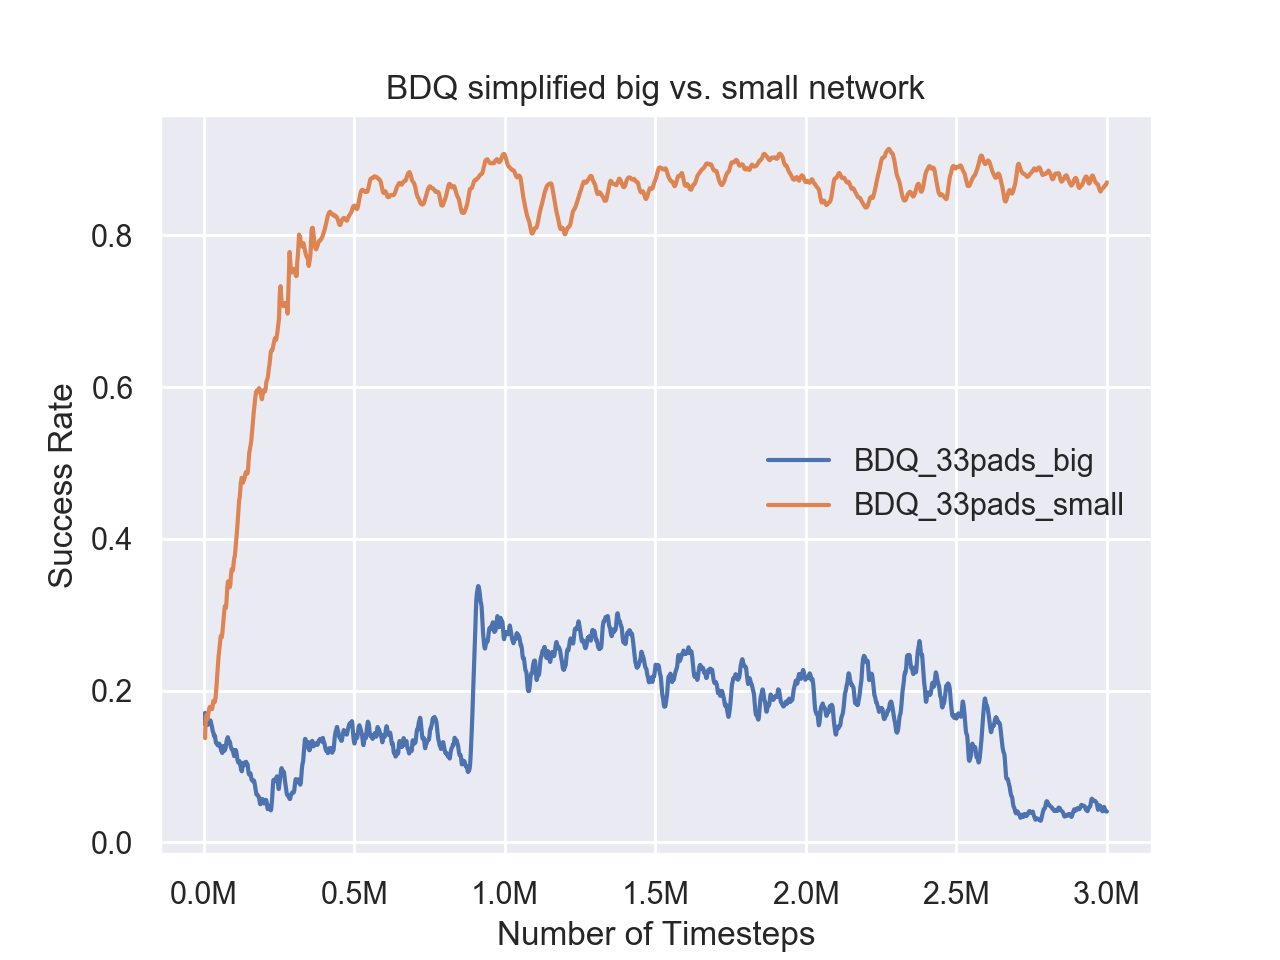
\includegraphics[width=\linewidth]{figures/BDQ_simplified_big_vs_small_network_no_var}
        \caption{Table Scene} \label{fig:table}
    \end{subfigure}%
    \hspace*{\fill}   % maximize separation between the subfigures
    \begin{subfigure}{0.49\textwidth}
        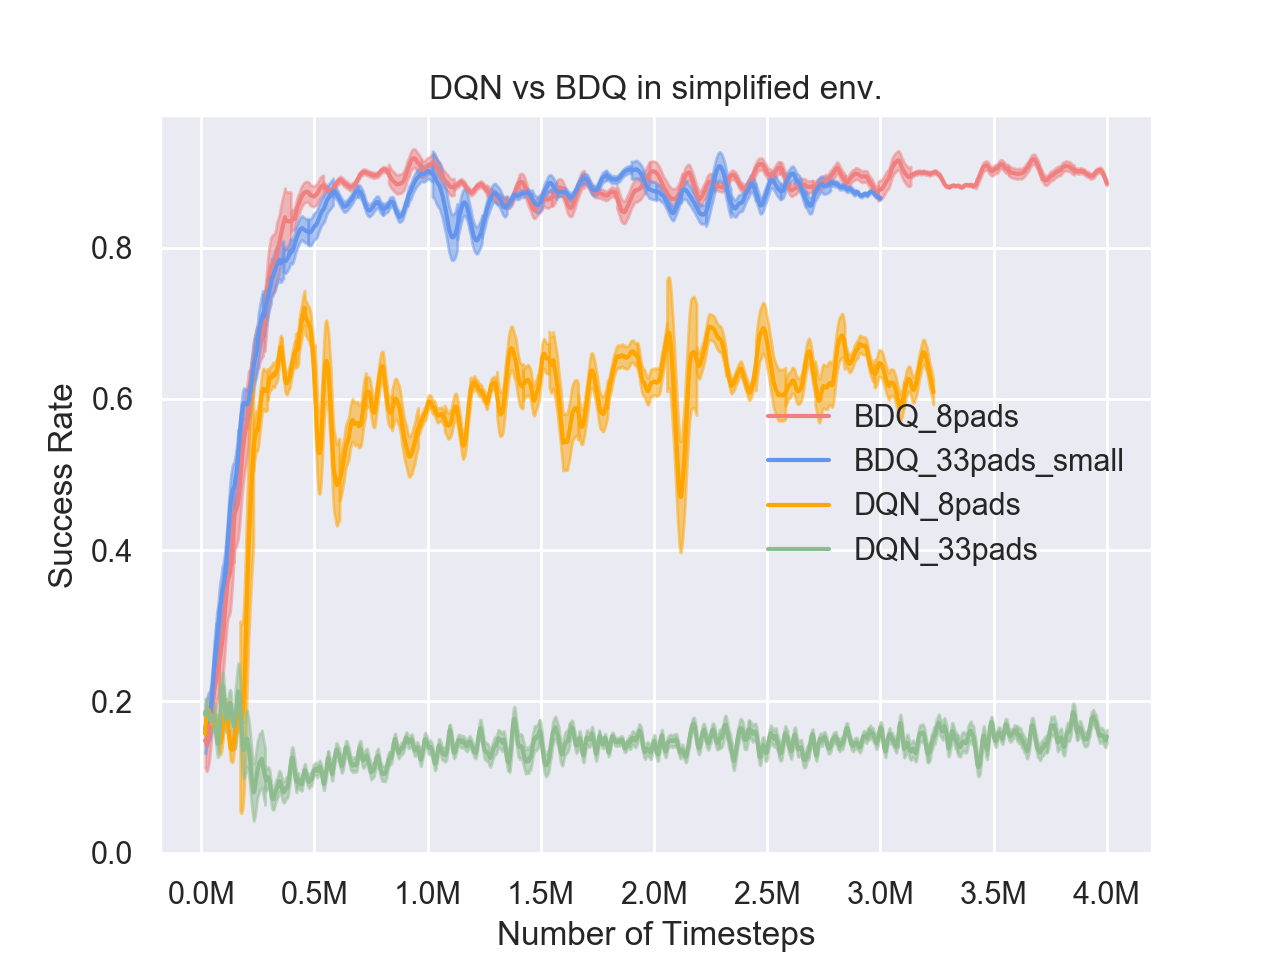
\includegraphics[width=\linewidth]{figures/DQN_vs_BDQ_in_simplified_env}
        \caption{Floor Scene} \label{fig:floor}
    \end{subfigure}%
    \hspace*{\fill}   % maximize separation between the subfigures


\caption{ Table and floor scenes \label{fig:scenes}}
\end{figure}

\begin{figure}[!htbp]
    \begin{subfigure}{0.49\textwidth}
        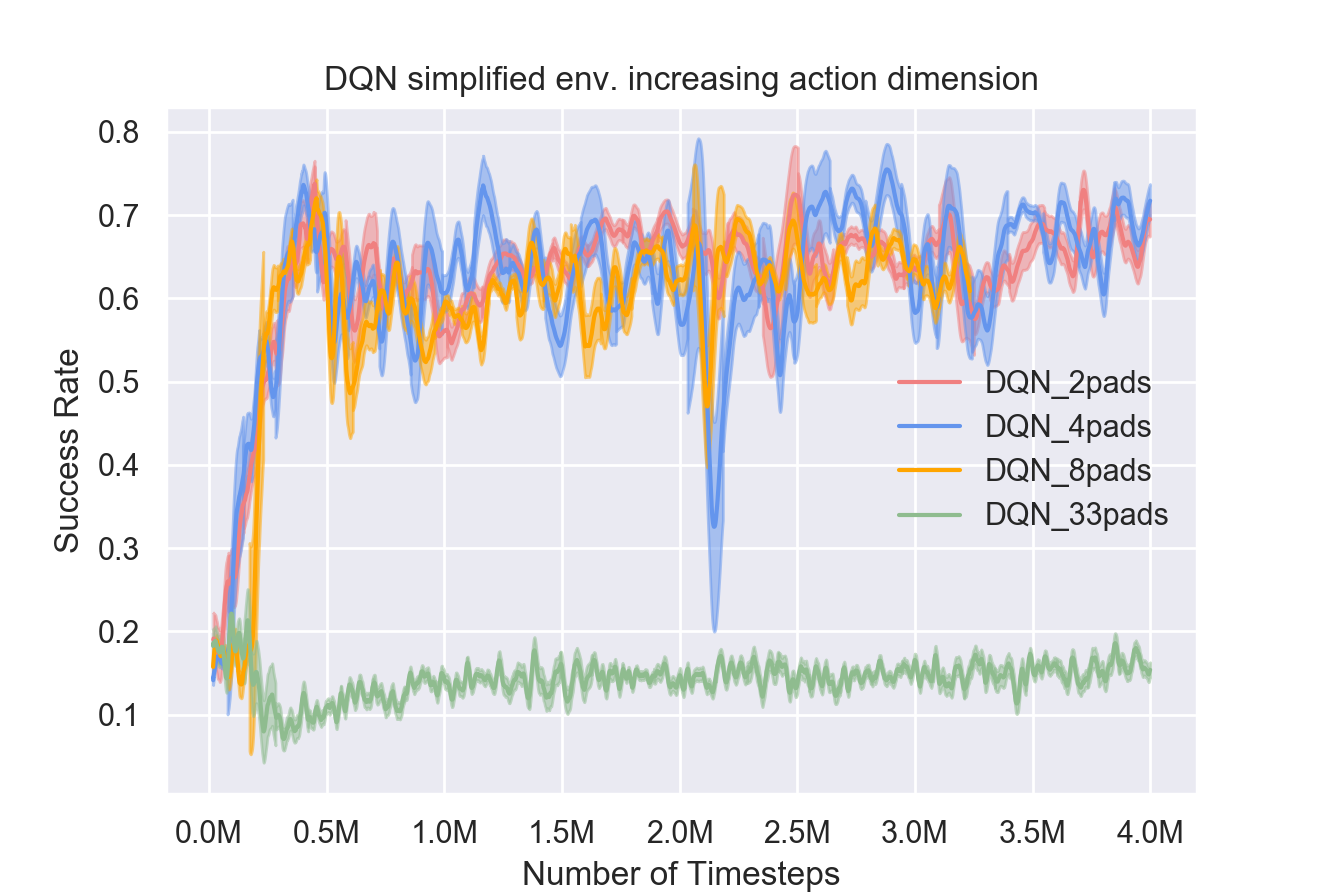
\includegraphics[width=\linewidth]{figures/DQN_simplified_env_increasing_action_dimension}
        \caption{Table Scene} \label{fig:table}
    \end{subfigure}%
    \hspace*{\fill}   % maximize separation between the subfigures
    \begin{subfigure}{0.49\textwidth}
        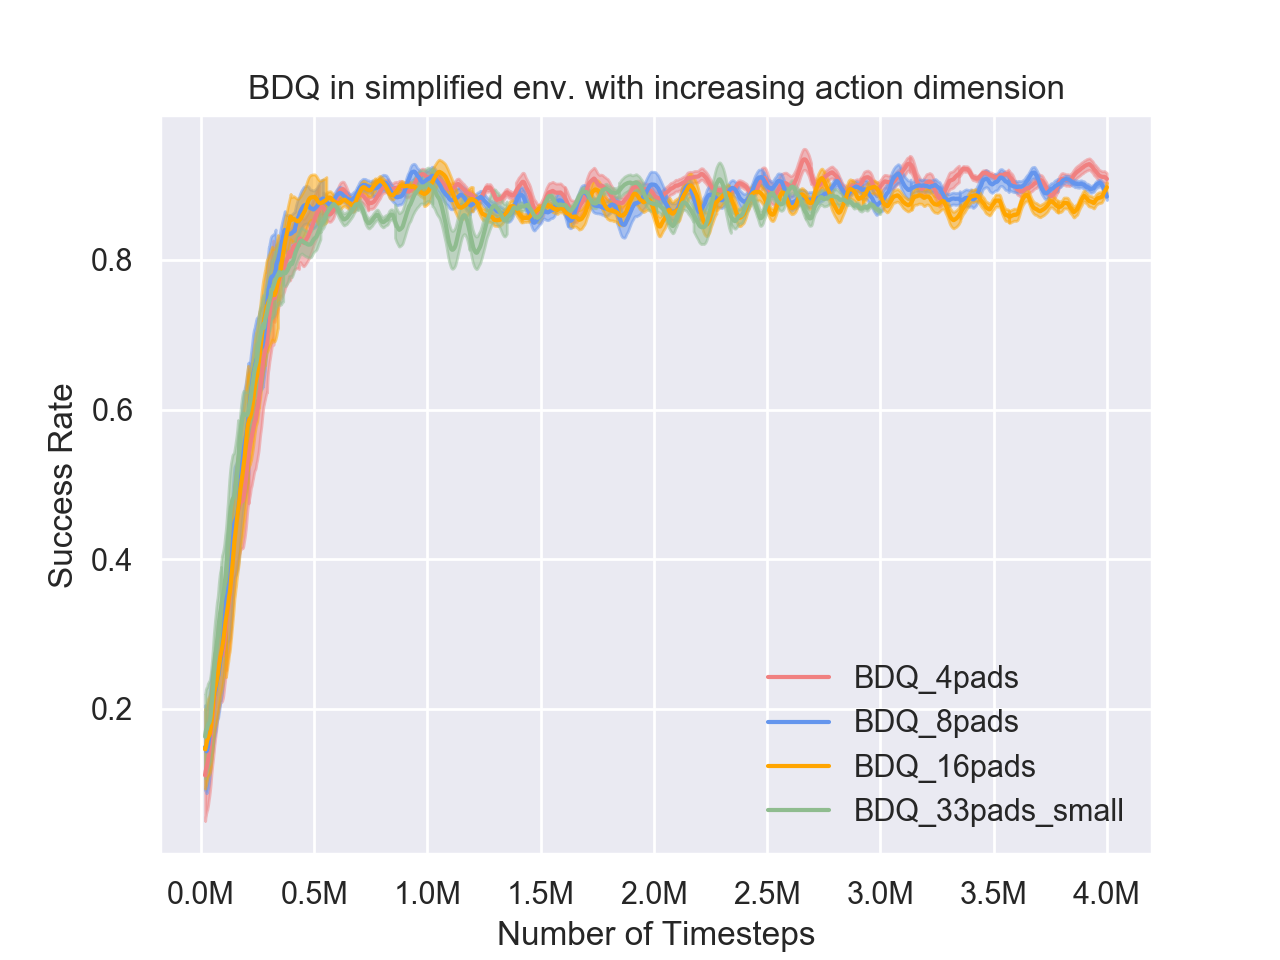
\includegraphics[width=\linewidth]{figures/BDQ_in_simplified_env_with_increasing_action_dimension}
        \caption{Floor Scene} \label{fig:floor}
    \end{subfigure}%
    \hspace*{\fill}   % maximize separation between the subfigures


\caption{ Table and floor scenes \label{fig:scenes}}
\end{figure}



\begin{figure}[!htbp]
    \begin{subfigure}{0.49\textwidth}
        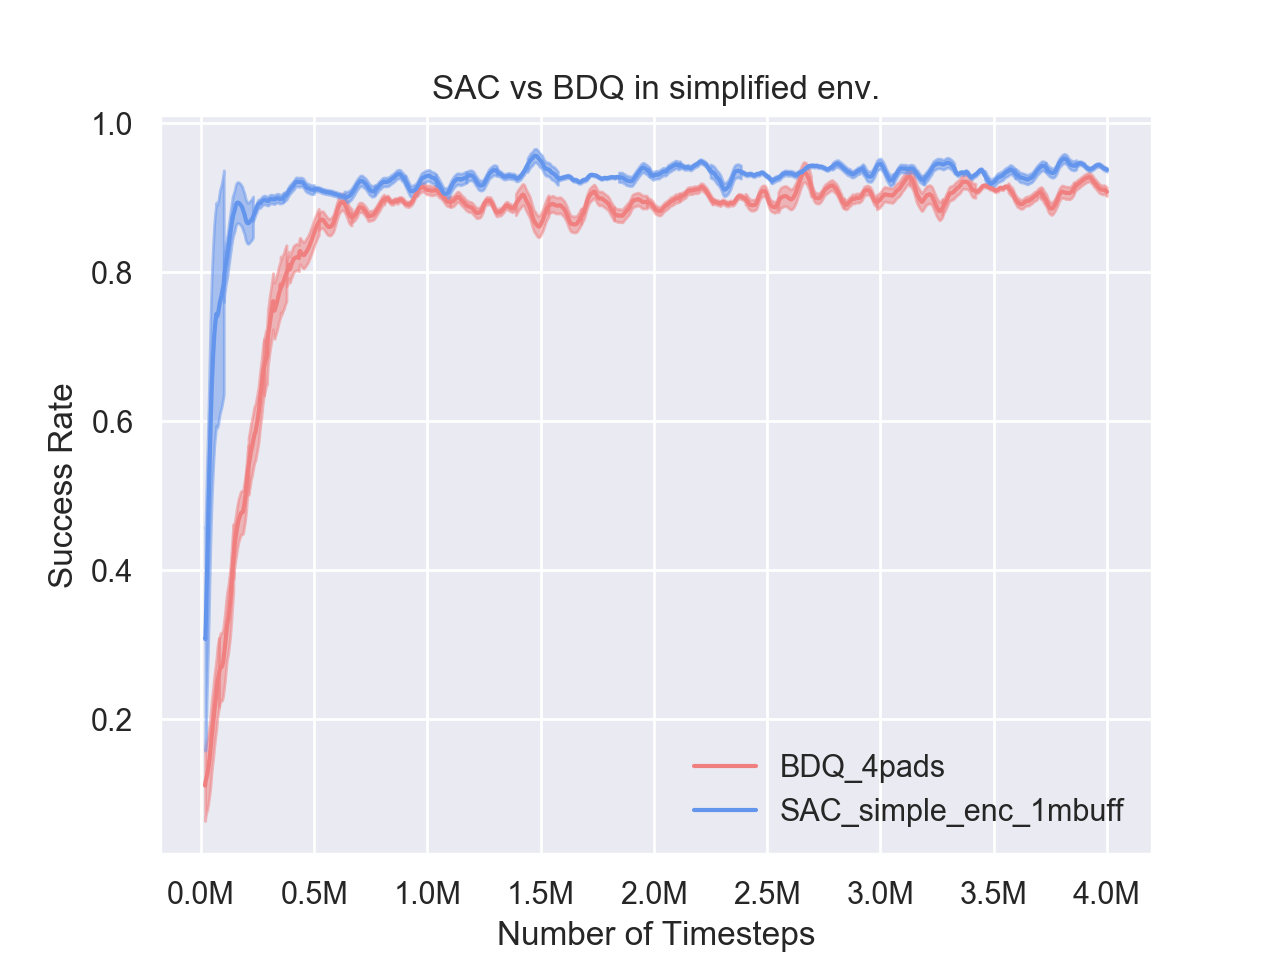
\includegraphics[width=\linewidth]{figures/SAC_vs_BDQ_in_simplified_env}
        \caption{Table Scene} \label{fig:table}
    \end{subfigure}%
    \hspace*{\fill}   % maximize separation between the subfigures
    \begin{subfigure}{0.49\textwidth}
        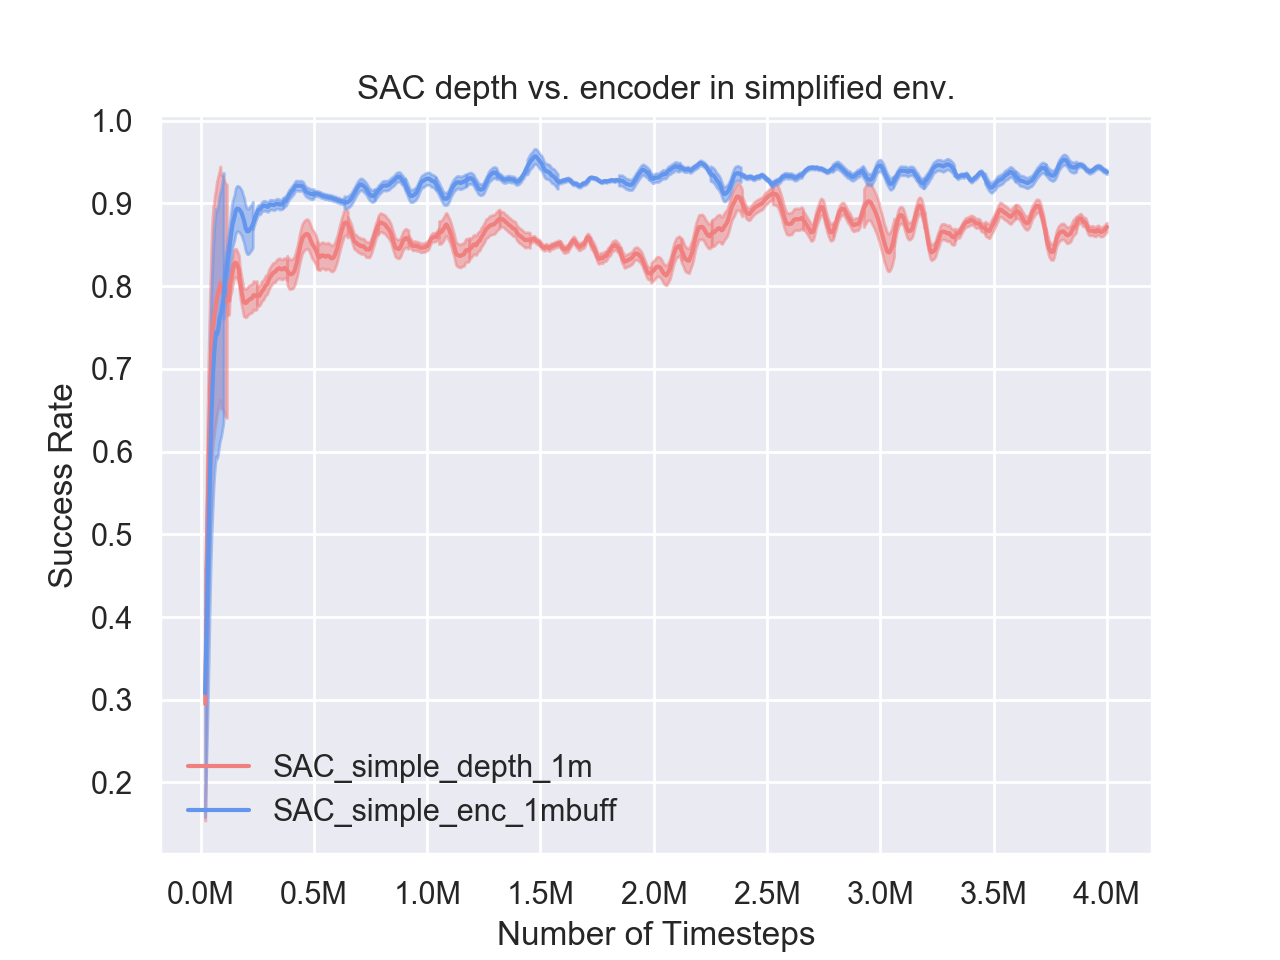
\includegraphics[width=\linewidth]{figures/SAC_depth_vs_encoder_in_simplified_env}
        \caption{Floor Scene} \label{fig:floor}
    \end{subfigure}%
    \hspace*{\fill}   % maximize separation between the subfigures


\caption{ Table and floor scenes \label{fig:scenes}}
\end{figure}

% \begin{figure}[!htbp]
%     \centering
%         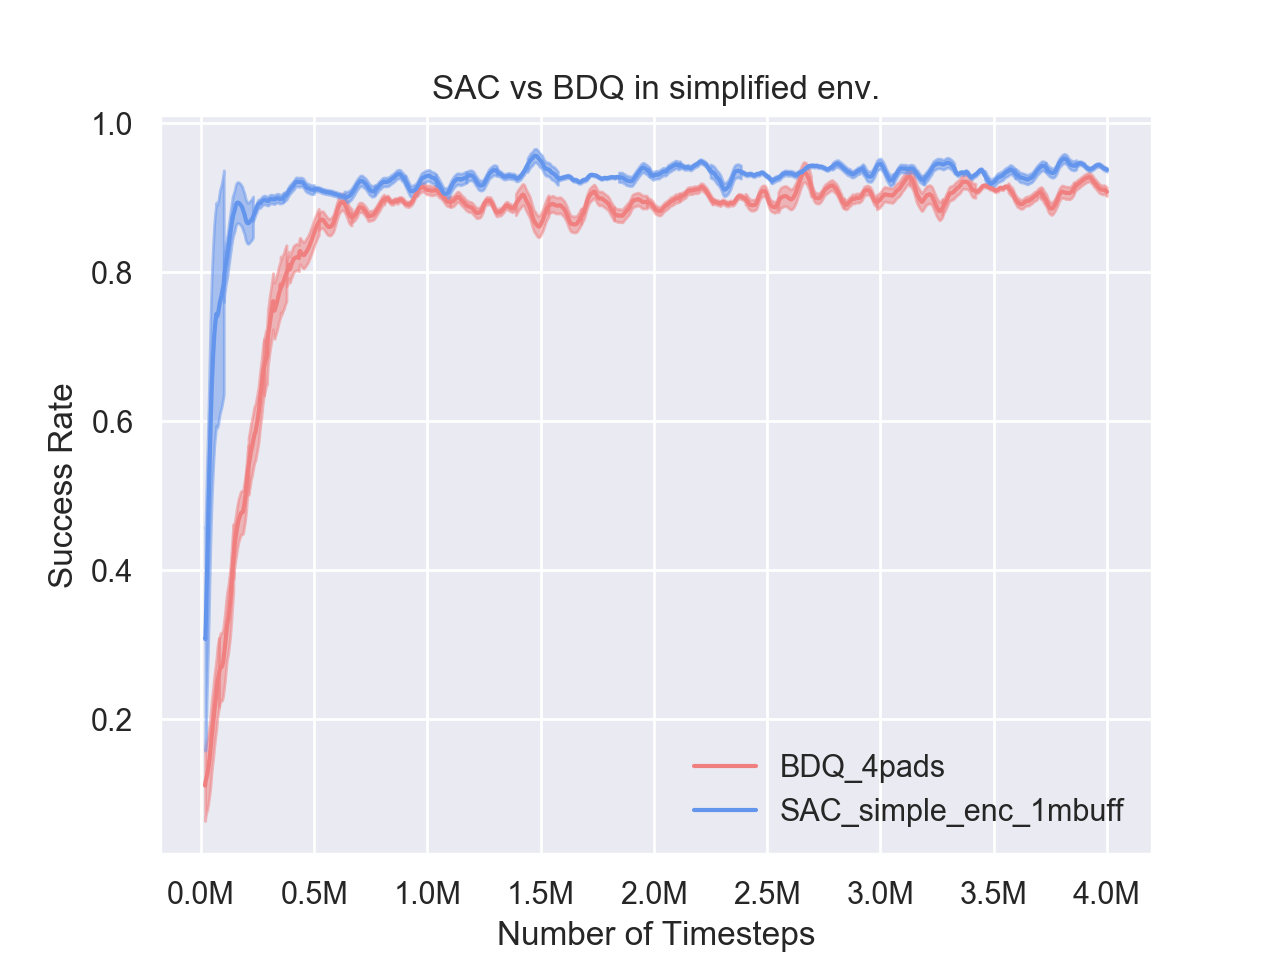
\includegraphics[width=0.4\textwidth]{figures/SAC_vs_BDQ_in_simplified_env}
%     \caption{Different manipulation skill adopted to robotic manipulators \cite{Kroemer2019}}
%     \label{fig:x manipulation_skills}
% \end{figure}

% \begin{figure}[!htbp]
%     \centering
%         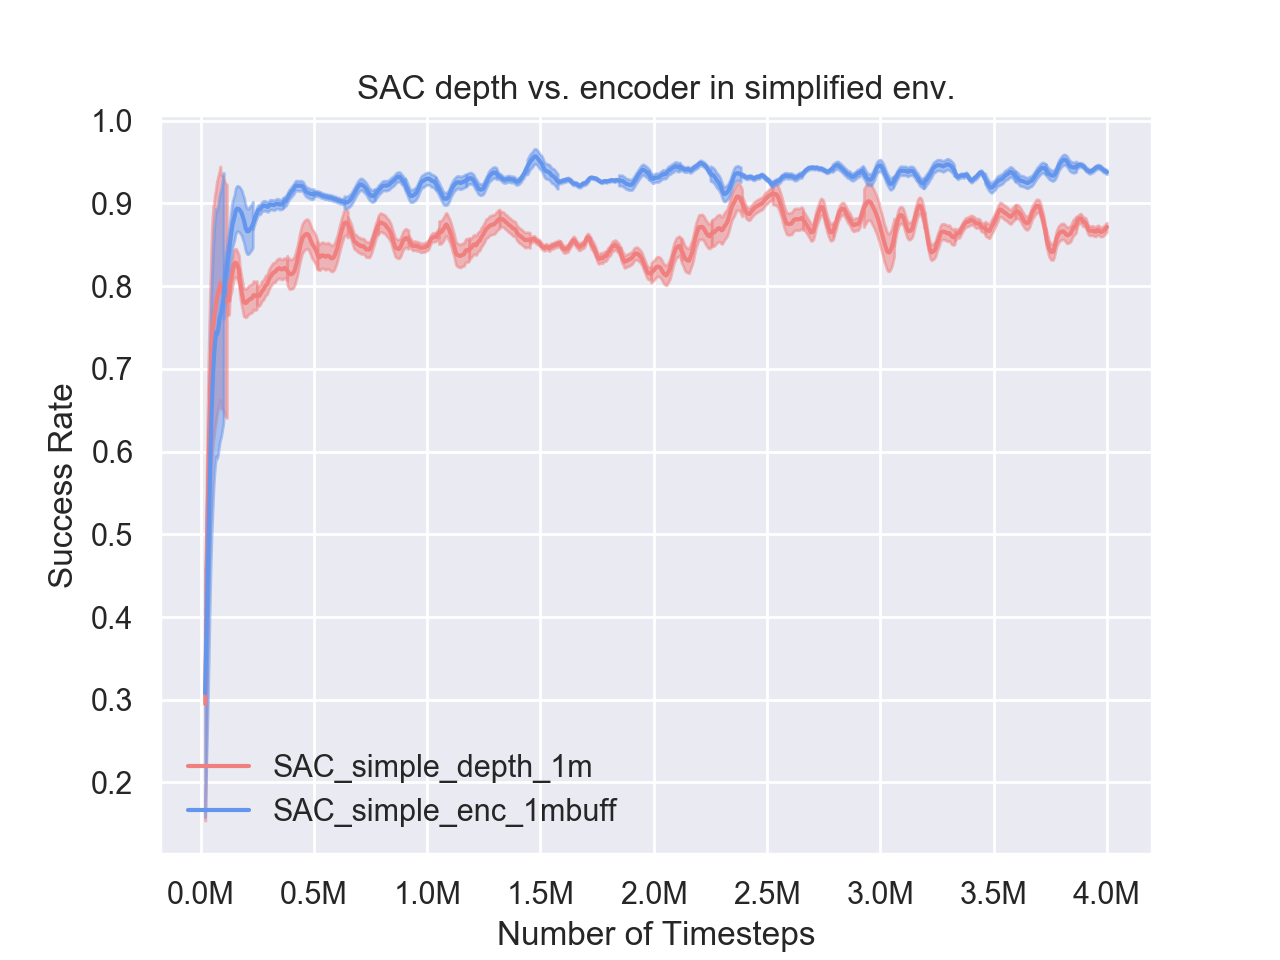
\includegraphics[width=0.4\textwidth]{figures/SAC_depth_vs_encoder_in_simplified_env}
%     \caption{Different manipulation skill adopted to robotic manipulators \cite{Kroemer2019}}
%     \label{fig:x manipulation_skills}
% \end{figure}



\section{Full Environment Results}


Among the three algorithms, only SAC delivered a working grasp policy. Therefore, we mostly evaluated the performance of the SAC algorithm's variants. We tested with different perception pipeline, different reward definition, and buffer size. Contrary to the simplified environment, we verified the algorithm's robustness on the wooden block object database. \todo{MORE}


\begin{table}[!htbp]
    \begin{tabular}{|l|l|l|l|l|}
    \hline
                                  & \multicolumn{4}{c|}{\textbf{SAC Full Environment}}                                                                                                                                                                                                                                                                                                                                  \\ \hline
                                  & \multicolumn{2}{c|}{\textbf{Floor Scene}}                                                                                                                                                & \multicolumn{2}{c|}{\textbf{Table Scene}}                                                                                                                                                \\ \hline
    \textbf{Models}               & \multicolumn{1}{c|}{\textbf{\begin{tabular}[c]{@{}c@{}}Random Objects\\ (\%)\end{tabular}}} & \multicolumn{1}{c|}{\textbf{\begin{tabular}[c]{@{}c@{}}Wooden Blocks\\ (\%)\end{tabular}}} & \multicolumn{1}{c|}{\textbf{\begin{tabular}[c]{@{}c@{}}Random Objects\\ (\%)\end{tabular}}} & \multicolumn{1}{c|}{\textbf{\begin{tabular}[c]{@{}c@{}}Wooden Blocks\\ (\%)\end{tabular}}} \\ \hline
    \textbf{SAC\_encoder\_50k}    & 65                                                                                          & 62                                                                                         & 63                                                                                          & 59                                                                                         \\ \hline
    \textbf{SAC\_encoder\_1m}     & 100                                                                                         & 95                                                                                         & 99                                                                                          & 82                                                                                         \\ \hline
    \textbf{SAC\_depth}           & 100                                                                                         & 95                                                                                         & 95                                                                                          & 23                                                                                         \\ \hline
    \textbf{SAC\_rgbd}            & 91                                                                                          & 95                                                                                         & 46                                                                                          & 17                                                                                         \\ \hline
    \textbf{SAC\_depth\_no\_curr} & 100                                                                                         & 97                                                                                         & 97                                                                                          & 64                                                                                         \\ \hline
    \textbf{SAC\_depth\_sparse}   & 99                                                                                          & 97                                                                                         & 100                                                                                         & 72                                                                                         \\ \hline
    \textbf{SAC\_depth\_no\_act}  & 95                                                                                          & 75                                                                                         & 84                                                                                          & 24                                                                                         \\ \hline
\end{tabular}
\end{table}


\begin{figure}[!htbp]
    \begin{subfigure}{0.49\textwidth}
        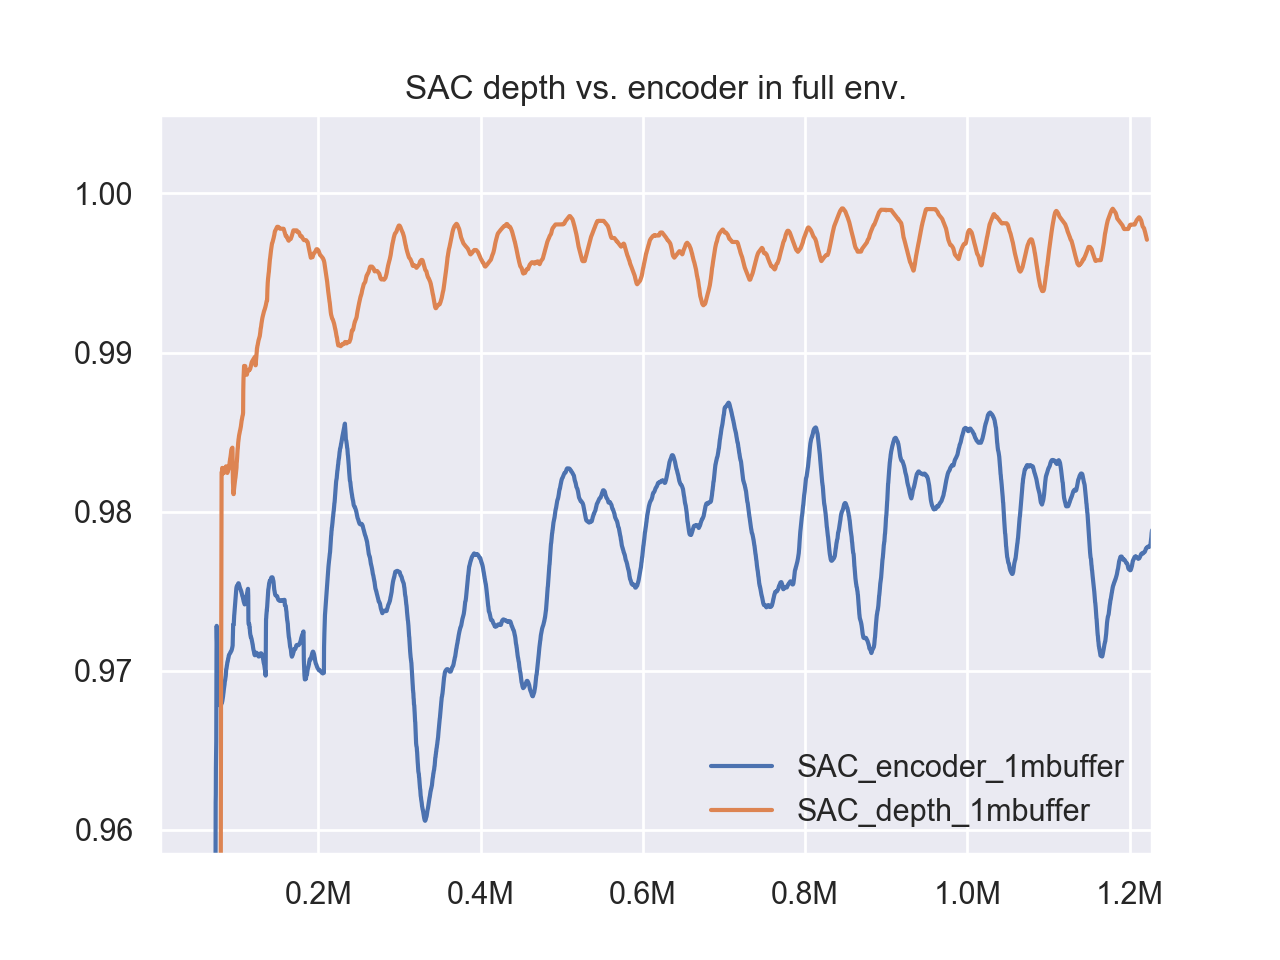
\includegraphics[width=\linewidth]{figures/SACfull/SAC_depth_vs_encoder_in_full_env}
        \caption{Table Scene} \label{fig:table}
    \end{subfigure}%
    \hspace*{\fill}   % maximize separation between the subfigures
    \begin{subfigure}{0.49\textwidth}
        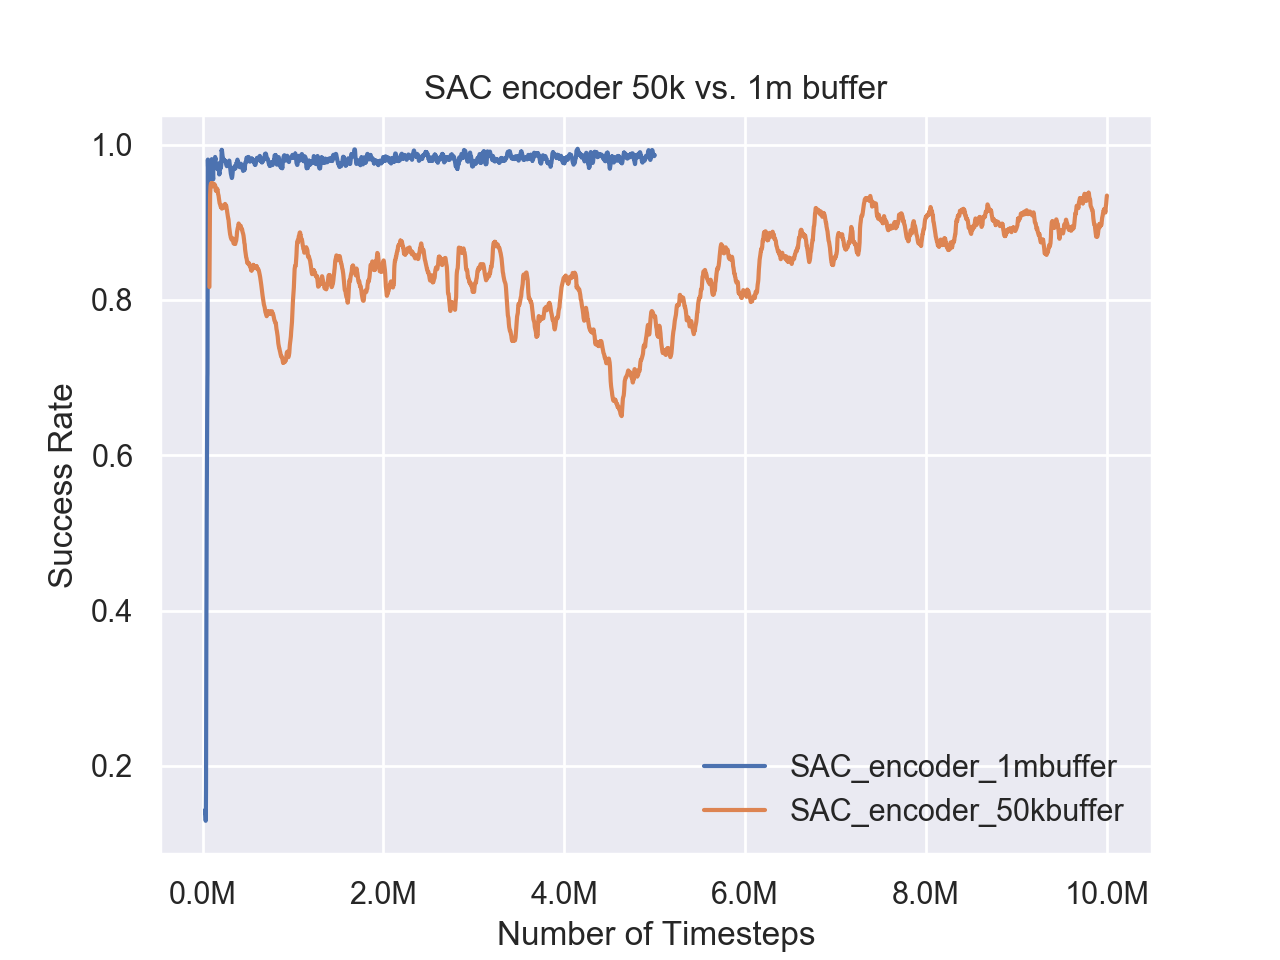
\includegraphics[width=\linewidth]{figures/SACfull/SAC_encoder_50k_vs_1m_buffer}
        \caption{Floor Scene} \label{fig:floor}
    \end{subfigure}%
    \hspace*{\fill}   % maximize separation between the subfigures


\caption{ Table and floor scenes \label{fig:scenes}}
\end{figure}

\begin{figure}[!htbp]
    \centering
        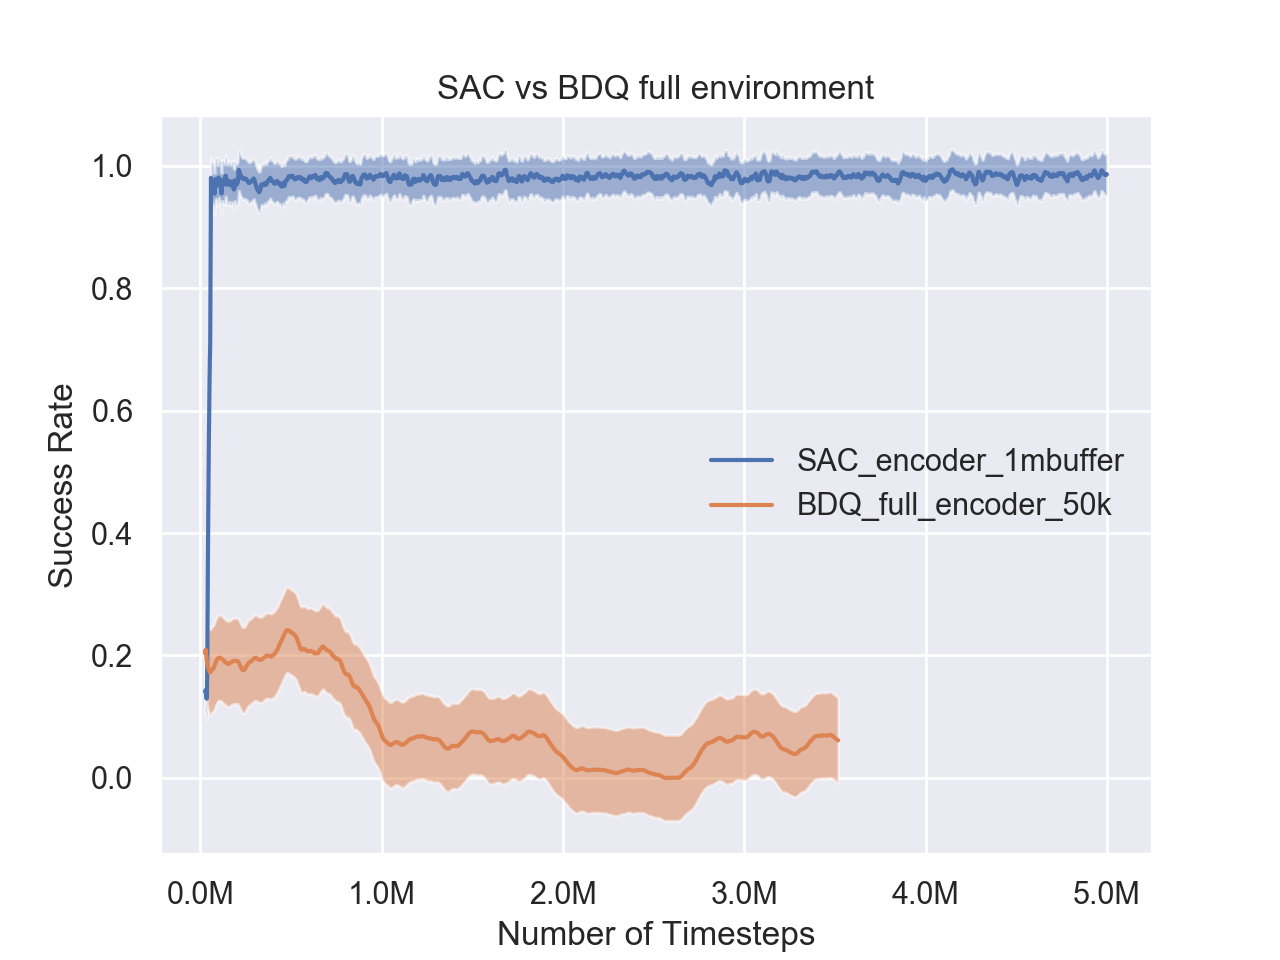
\includegraphics[width=0.4\textwidth]{figures/SACfull/SAC_vs_BDQ_full_environment}
    \caption{Different manipulation skill adopted to robotic manipulators \cite{Kroemer2019}}
    \label{fig:x manipulation_skills}
\end{figure}


\section{Ablation Studies}

In ablation studies, we investigated the individual importance of the following modules: curriculum strategy, input and reward normalization, actuator-width information, and the shaped reward. All ablation study experiments were carried with the SAC algorithm with depth perception and one million experience replay buffer size. All training trials took place in the full environment floor scene. We shared the results of ablation studies in the same table as the SAC full environment \ref{table:SACfull}.

Among all ablation variants, only no normalization trial did not provide a working grasp policy. The rest either converged to a lower success rate or converged relatively slower than the baseline. 

Sparse reward and no curriculum learning converged 20 thousand timesteps and 400 thousand timesteps after the baselines. Interestingly, sparse reward SAC agent performed the best in the table scene, on random objects with a 100\% success rate. Both sparse and no curriculum learning trials performed better than the baseline SAC model on wooden blocks in the table scene. Sparse reward and no curriculum learning achieved 72\% and 64\%, while baseline reached 23\%.

No actuator width observation converged to a slightly worse success rate than the baseline.  It achieved a 97\% success rate, while the baseline converged to 99\%. An extra observation related to the environment proved to be useful.

\begin{figure}[htbp]
    \begin{subfigure}{0.49\textwidth}
        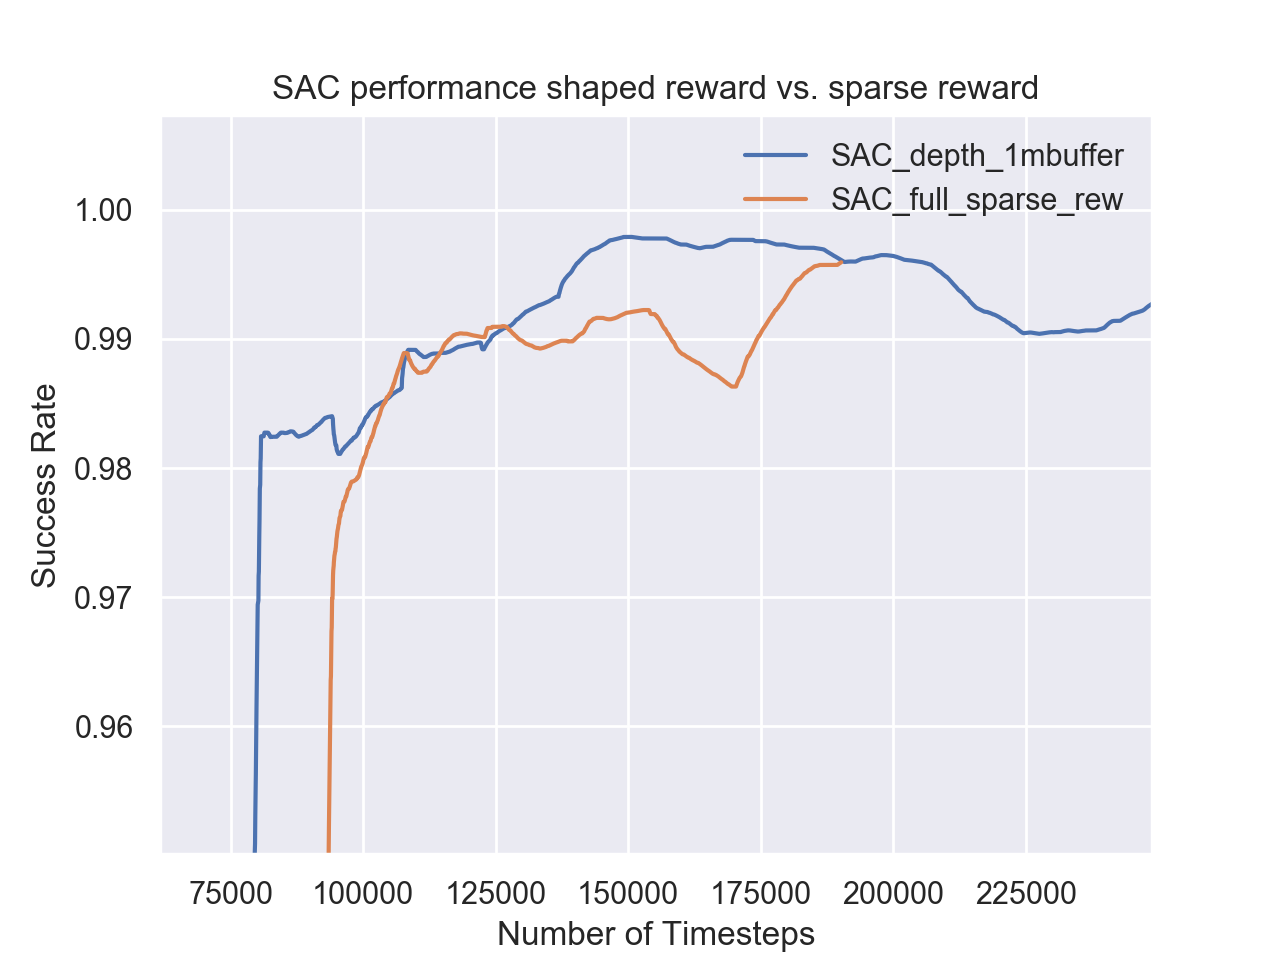
\includegraphics[width=\linewidth]{figures/ablation/SAC_performance_shaped_reward_vs_sparse_reward}
        \caption{SAC performance with shaped reward vs. sparse reward } \label{fig:table}
    \end{subfigure}%
    \hspace*{\fill}   % maximize separation between the subfigures
    \begin{subfigure}{0.49\textwidth}
        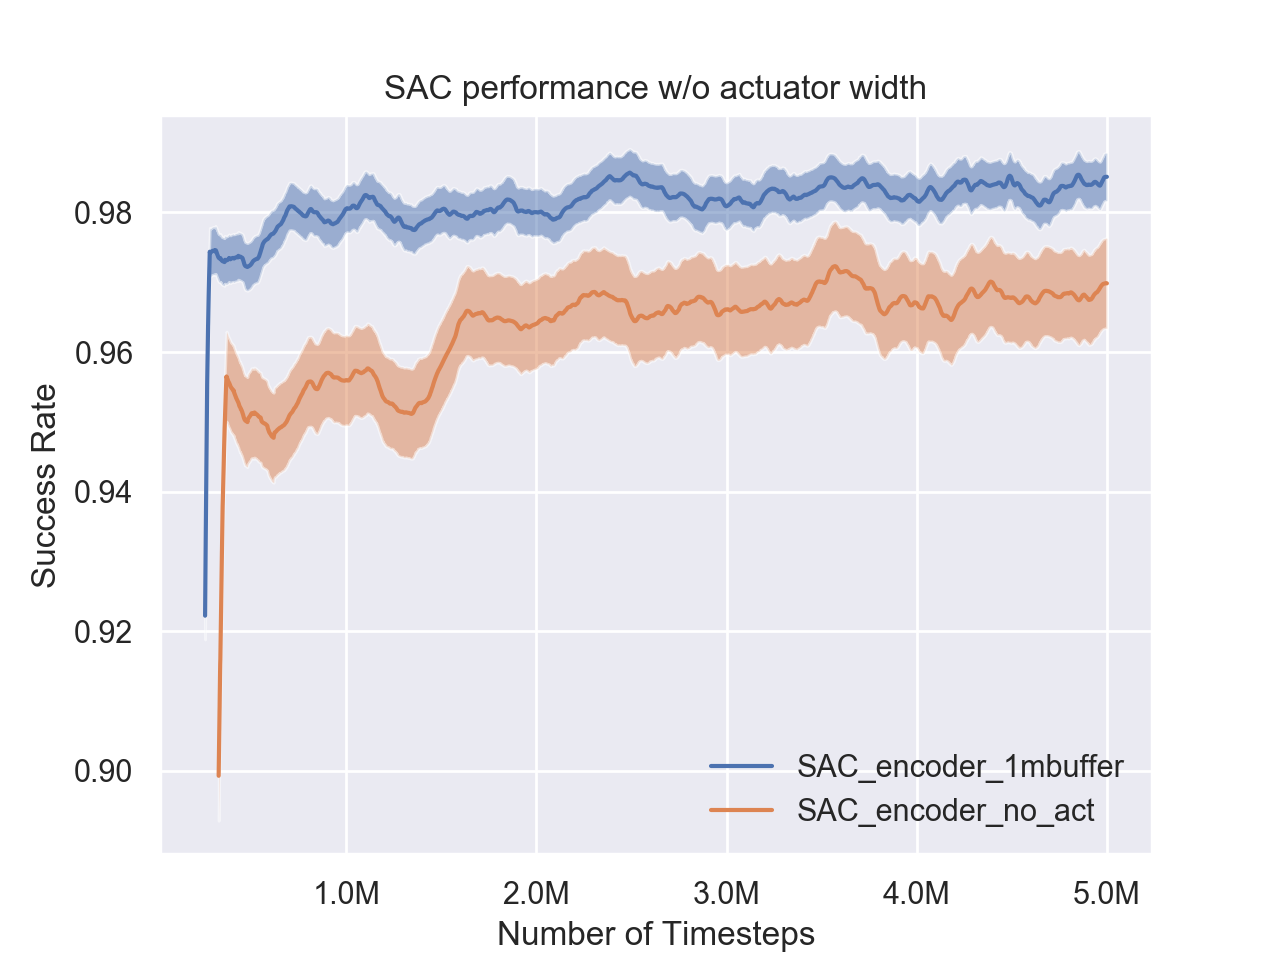
\includegraphics[width=\linewidth]{figures/ablation/SAC_performance_wo_actuator_width}
        \caption{SAC performance with encoder perception without actuator width observation} \label{fig:noact}
    \end{subfigure}%
    \hspace*{\fill}   % maximize separation between the subfigures


\caption{ Ablation of reward function and actuator width observation \label{fig:scenes}}
\end{figure}

\begin{figure}[htbp]
    \begin{subfigure}{0.49\textwidth}
        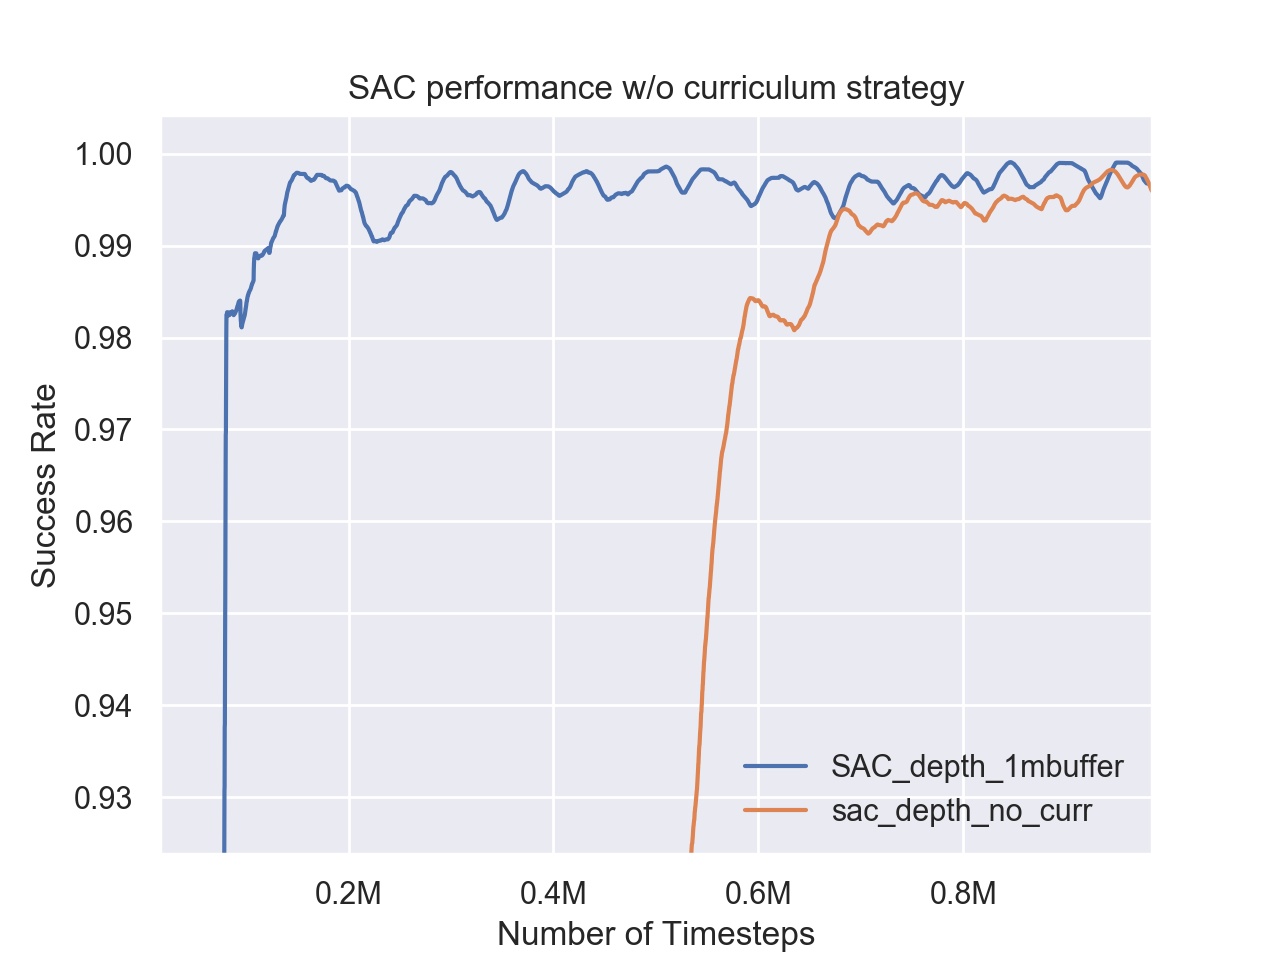
\includegraphics[width=\linewidth]{figures/ablation/SAC_performance_wo_curriculum_strategy}
        \caption{SAC performance withuot curriculum strategy} \label{fig:table}
    \end{subfigure}%
    \hspace*{\fill}   % maximize separation between the subfigures
    \begin{subfigure}{0.49\textwidth}
        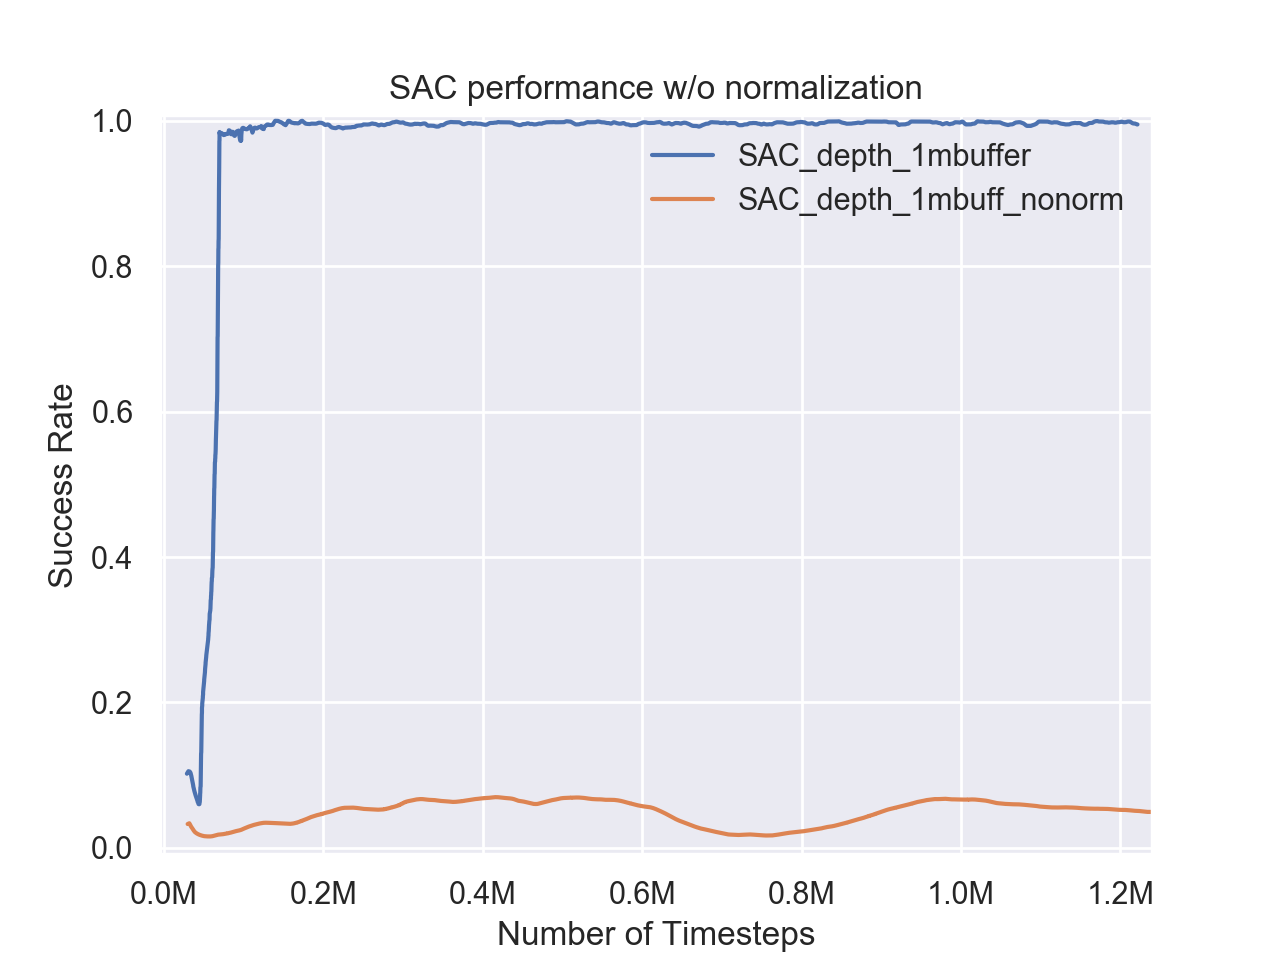
\includegraphics[width=\linewidth]{figures/ablation/SAC_performance_wo_normalization}
        \caption{SAC performance in full environment without normalization compared to the performance of the baseline SAC} \label{fig:nonorm}
    \end{subfigure}%
    \hspace*{\fill}   % maximize separation between the subfigures


\caption{ Ablation of curriculum learning and normalization of input and reward \label{fig:scenes}}
\end{figure}





\section{Failure Modes \label{sec:fail}}


\begin{enumerate}
    \item \textbf{Misinterpretation of Depth} - One of the most common failure case of encoder perception pipeline is the misinterpretation of the depth. As shown in the figures at 
    \ref{fig:scenes}, the gripper orients itself correctly and position just a bit higher than the targeted object. After the positioning, it attempts to grasp the object but fails because of the height difference between the object and gripper. This scenario occurs more frequently in the test dataset than the training set. Agent can actually overcome this failure case by understanding that the encoder is yielding wrong information and it needs to go further down to grasp the object. However, since it does not have any knowledge about the test objects it tries the standard grasp policy but fails because of the discrepancy between encoded depth and real depth. That is the reason why the encoder converged to a lower success rate than the depth.
        % \begin{figure}[!htbp]
        %     \begin{subfigure}{0.49\textwidth}
        %         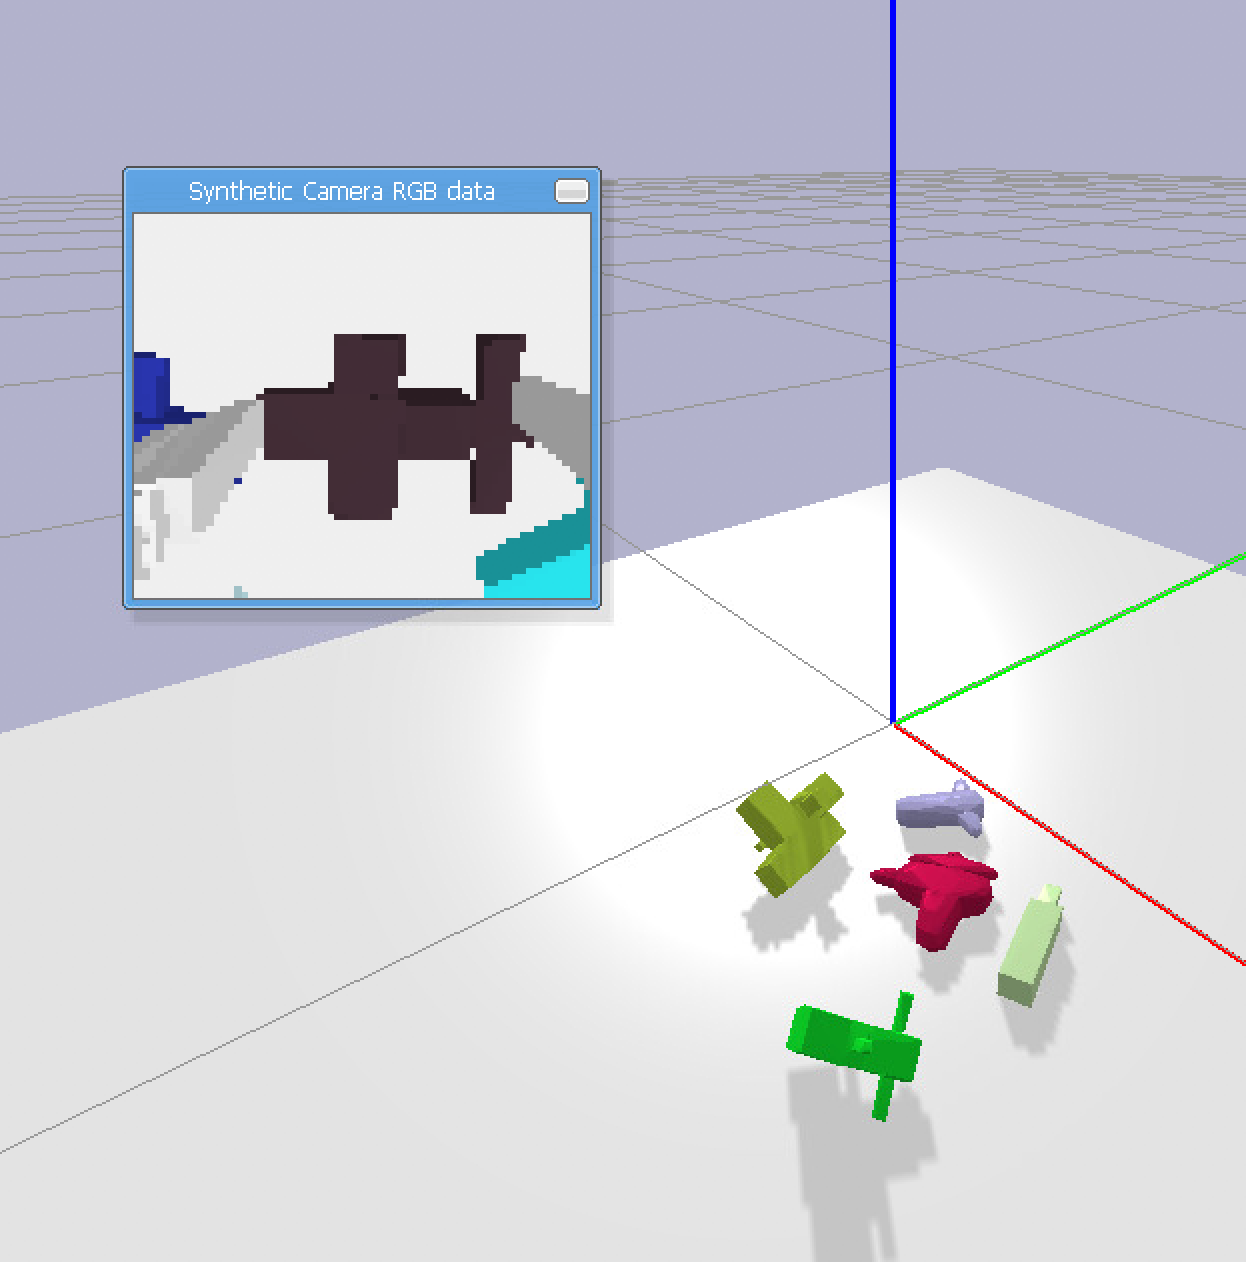
\includegraphics[width=\linewidth]{figures/failure/floorfailure1}
        %         \caption{Table Scene} \label{fig:table}
        %     \end{subfigure}%
        %     \hspace*{\fill}   % maximize separation between the subfigures
        %     \begin{subfigure}{0.49\textwidth}
        %         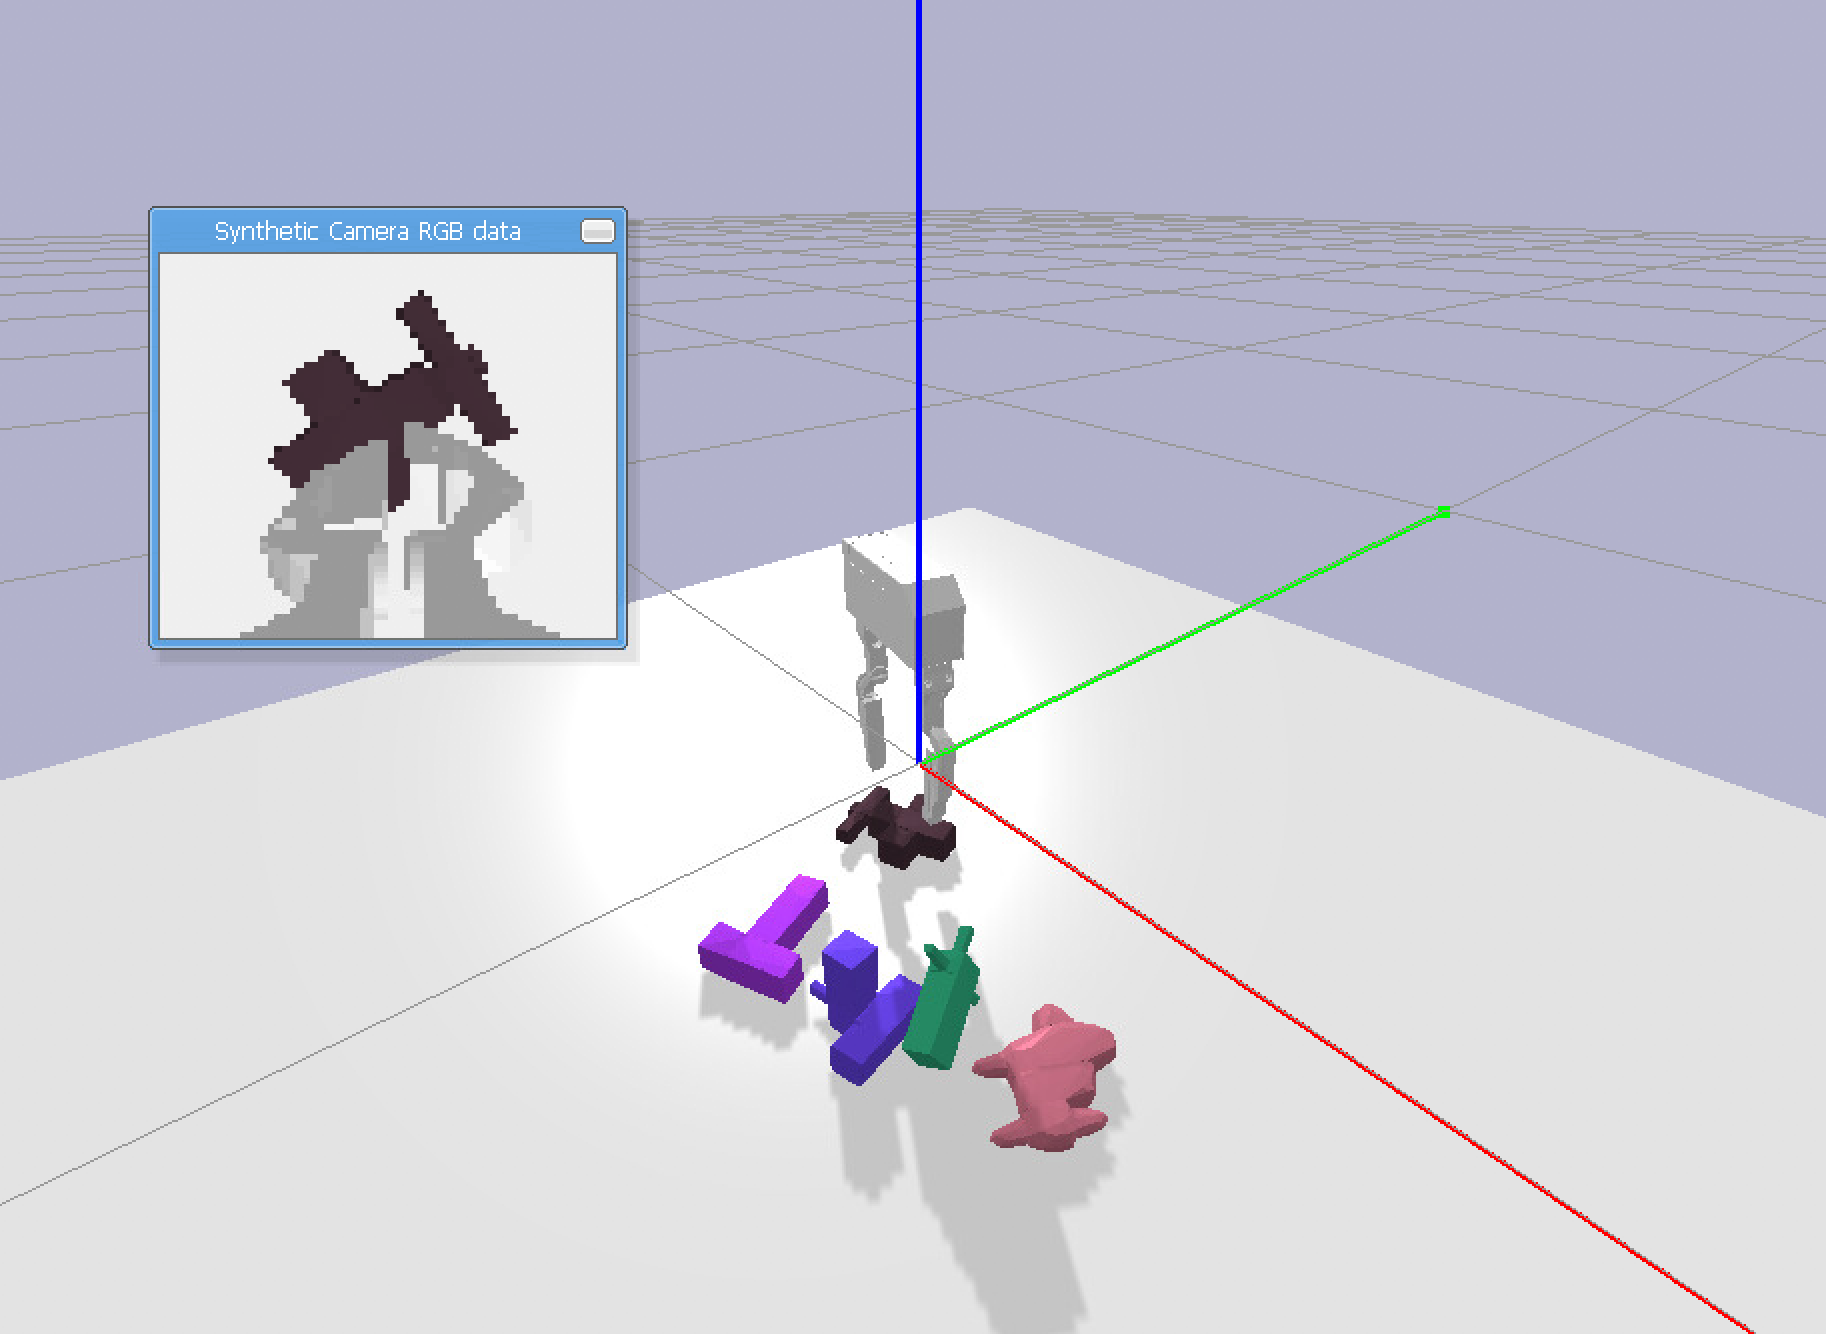
\includegraphics[width=\linewidth]{figures/failure/floorfailure2}
        %         \caption{Floor Scene} \label{fig:floor}
        %     \end{subfigure}%
        %     \hspace*{\fill}   % maximize separation between the subfigures    
        %     \caption{ Table and floor scenes \label{fig:scenes}}
        % \end{figure}
        \begin{figure}[!htbp]
            \begin{subfigure}{0.49\textwidth}
                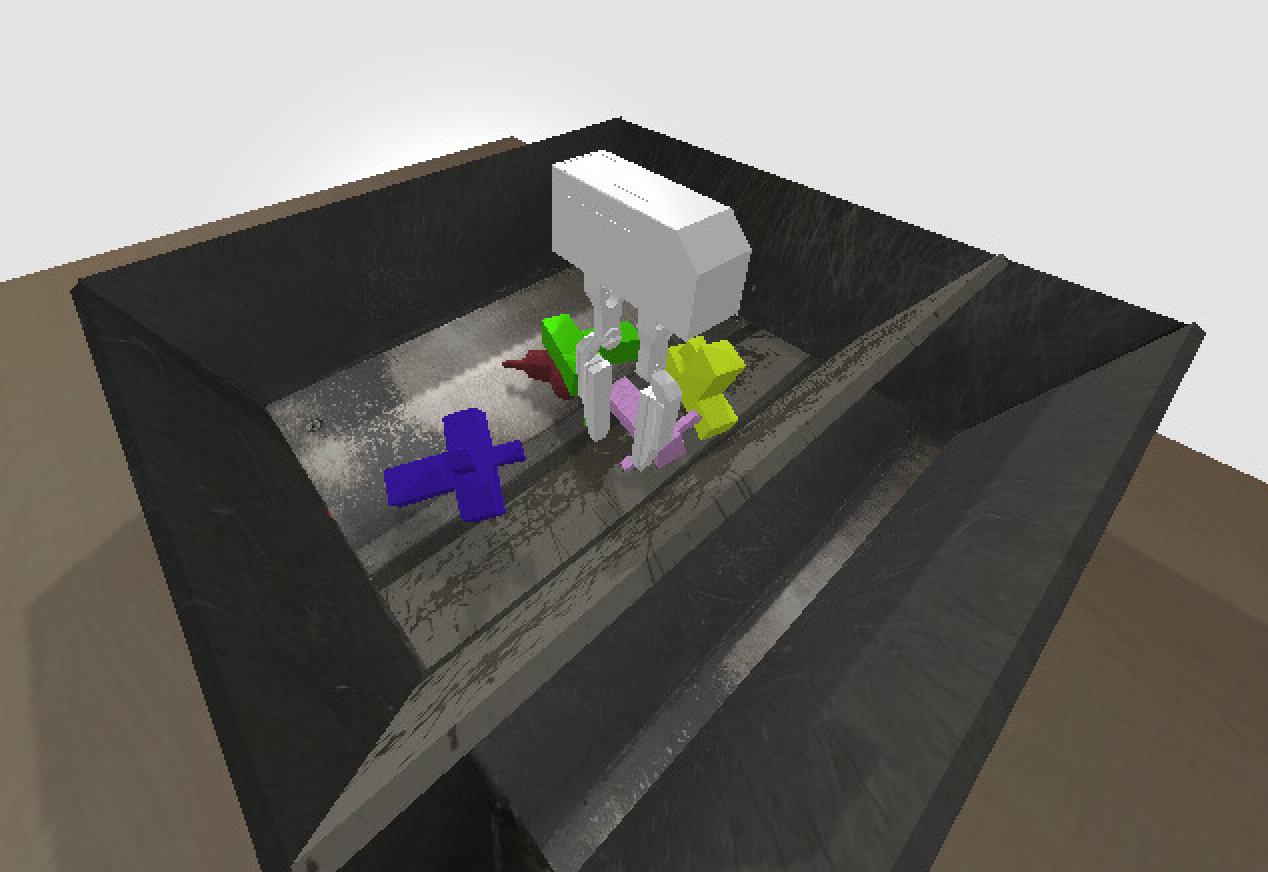
\includegraphics[width=\linewidth]{figures/failure/tablefailure2}
                \caption{Gripper positions itself above the pink object} \label{fig:table}
            \end{subfigure}%
            \hspace*{\fill}   % maximize separation between the subfigures
            \begin{subfigure}{0.49\textwidth}
                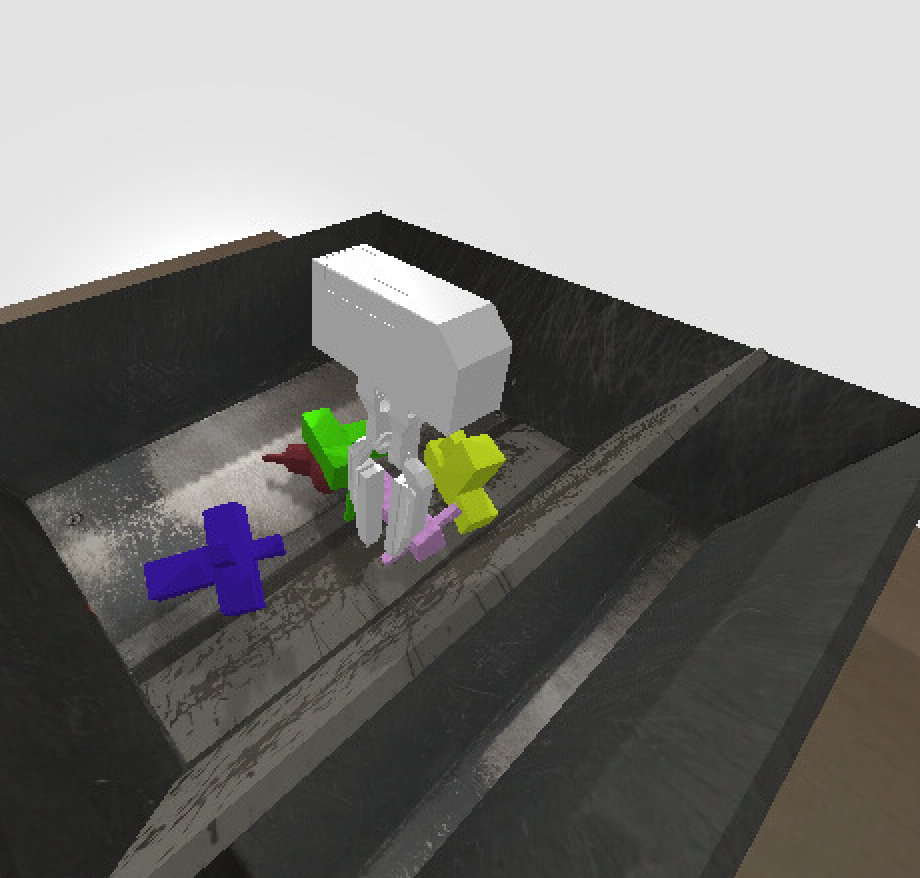
\includegraphics[width=\linewidth]{figures/failure/tablefailure1}
                \caption{Gripper attempts to grasp the pink object unsuccessfully} \label{fig:floor}
            \end{subfigure}%
            \hspace*{\fill}   % maximize separation between the subfigures    
            \caption{ Depth Misinterpretation of pink object in the full environment\label{fig:scenes}}
        \end{figure}

    \item \textbf{Grasping the tray's edge} - RGBD or Depth observation types perceive the tray's edge as an object. This misjudgment accounts for up to 50\% of the failed grasp attempts in the table scene \ref{table:SACfull} \ref{fig:failTrayEdge}. We realized that the failure percentage increases when we start the gripper from a higher start point.

    Both observation types tackled the height problem that appeared in the encoder problem. The online nature of these observation types corrected itself when a depth discrepancy occurs. However, it seems that these online observation methods encode the graspable objects' features very similar to other household objects. This characteristic can be interpreted both positively and negatively. It is positive because the perception layer extrapolates the graspable features correctly from the trained objects, and applies it correctly to the tray object. It can be viewed negatively because the tray is not our target object; eventually, the gripper should differentiate between the targeted objects and the extra tray object.   
    
    This failure mode can be solved by training the trained model for a short time in the table scene. This procedure should suffice for the agent to understand the tray is not the targeted object.
    \begin{figure}[!htbp]
        \begin{subfigure}{0.33\textwidth}
            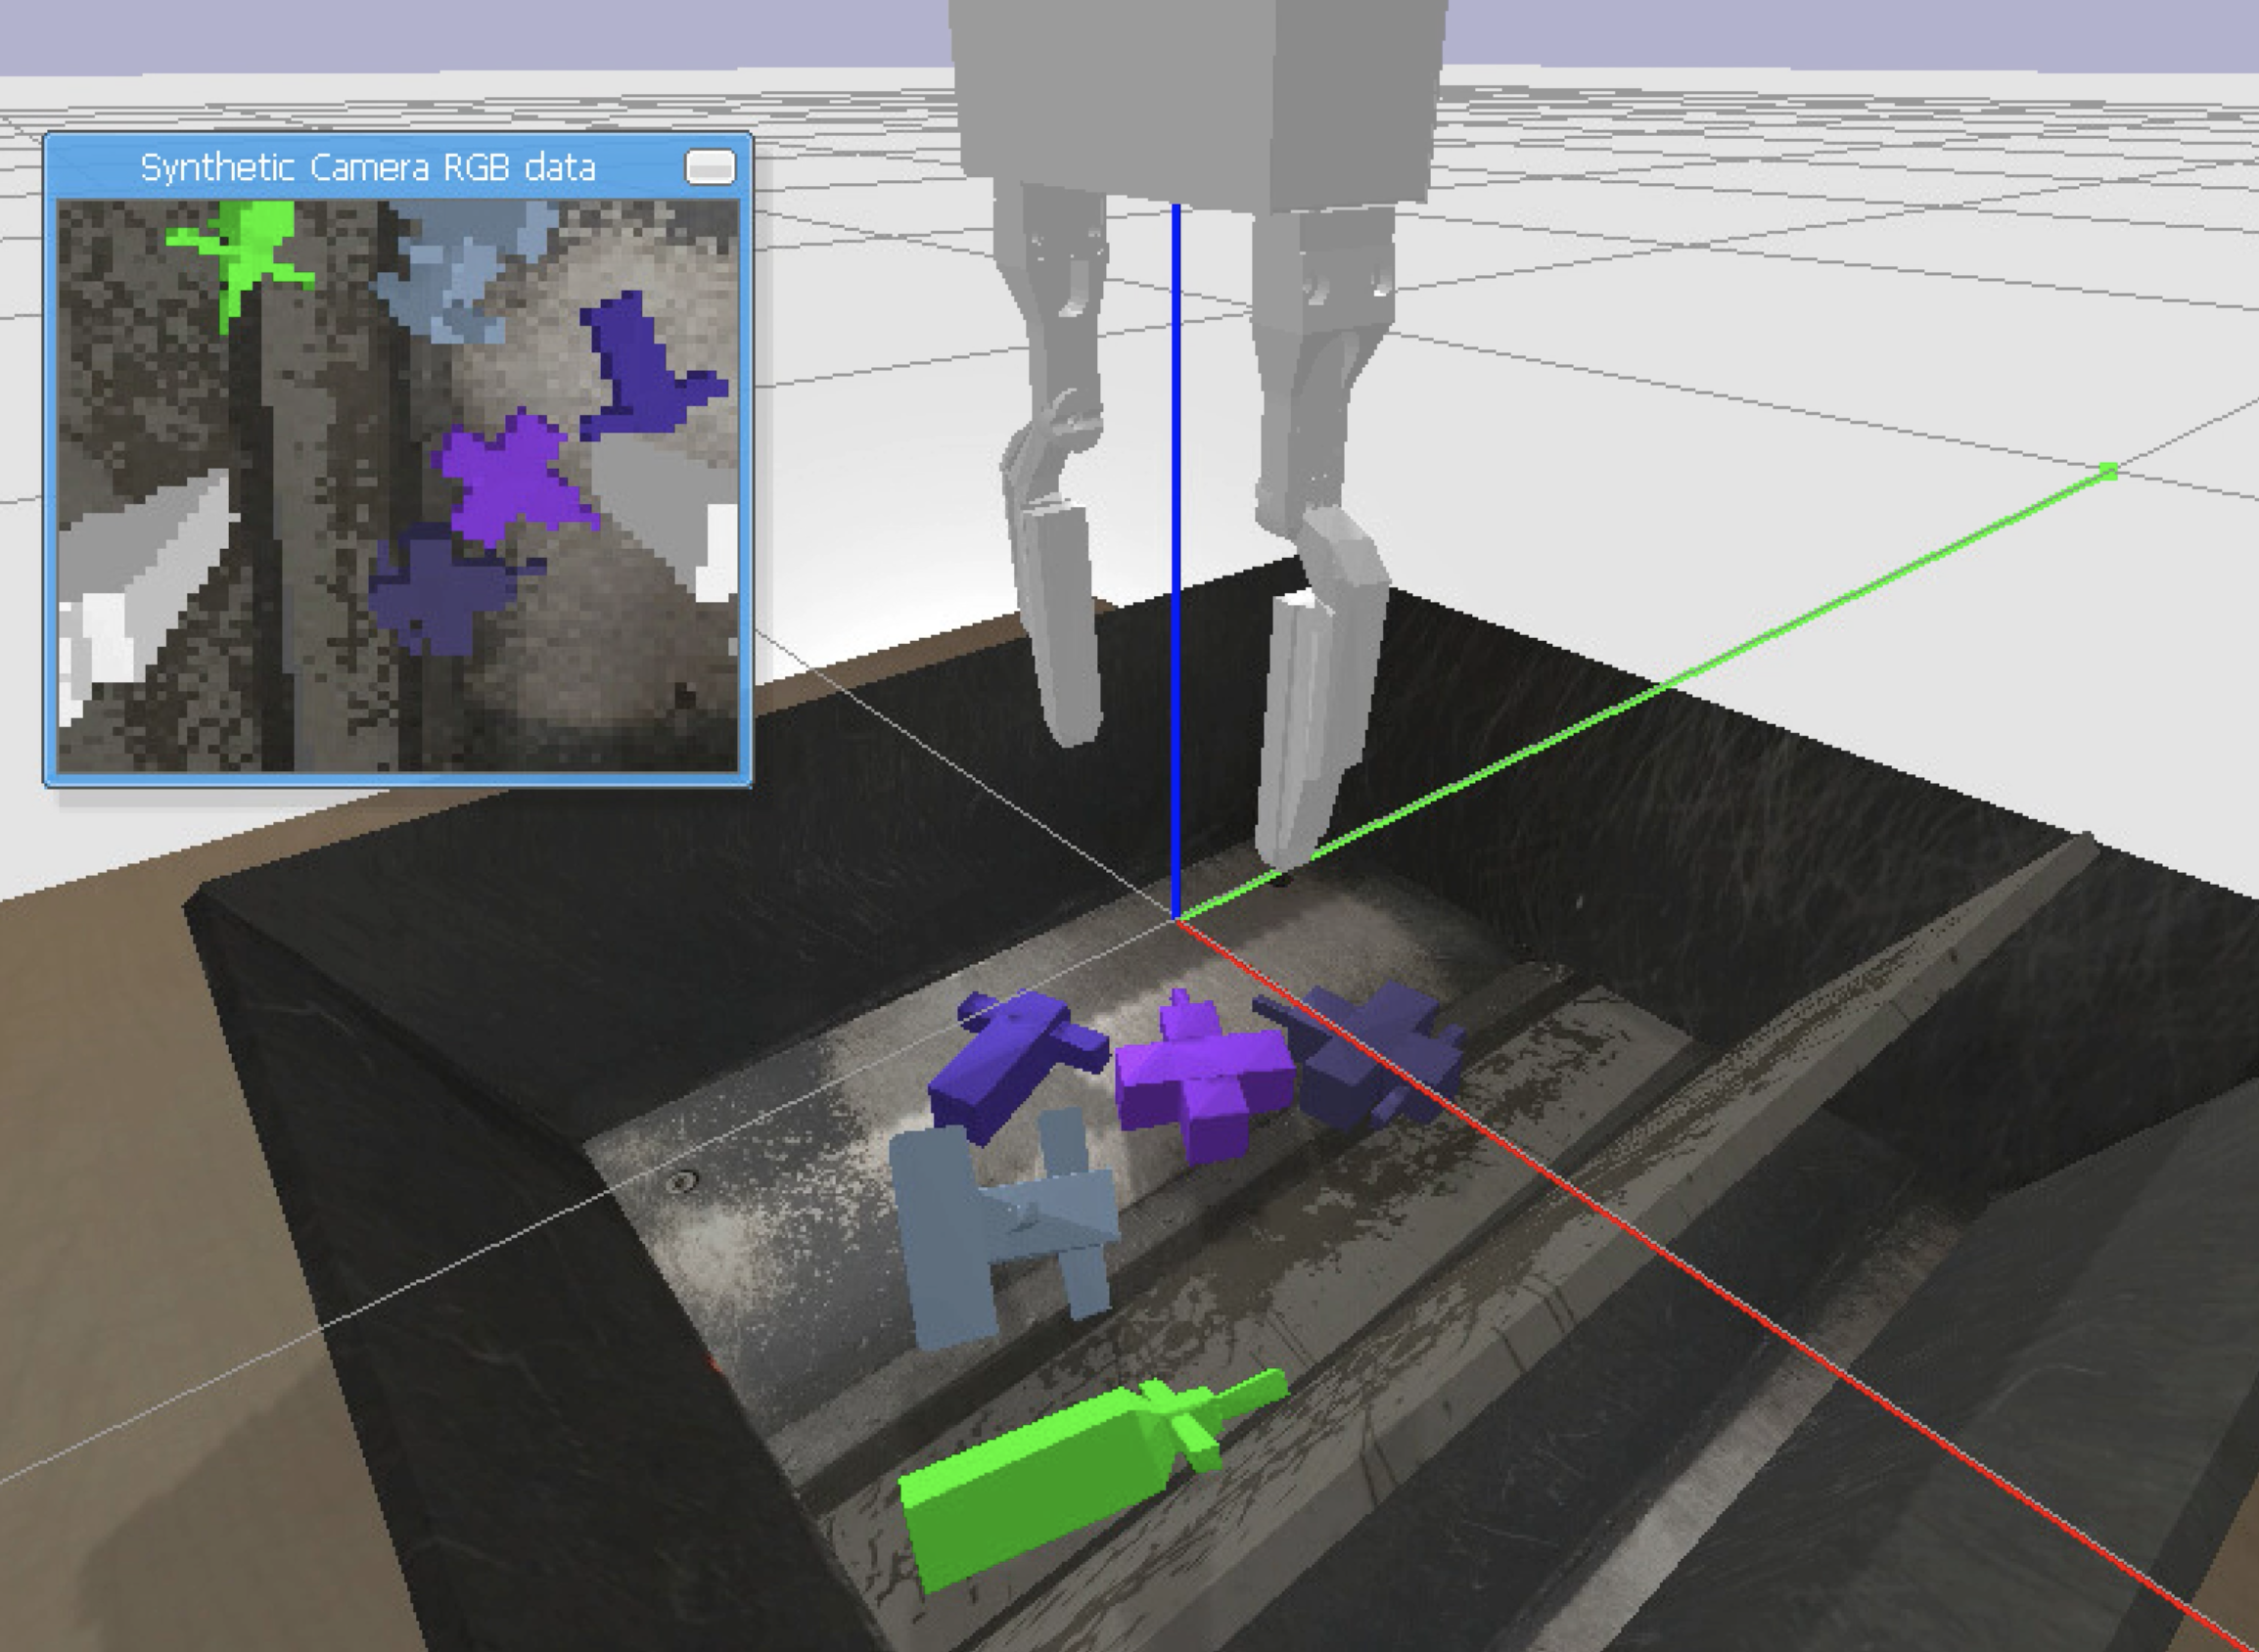
\includegraphics[width=\linewidth]{figures/failure/trayedge1}
            \caption{Gripper starts the movement to the tray's edge} \label{fig:table}
        \end{subfigure}%
        \hspace*{\fill}   % maximize separation between the subfigures
        \begin{subfigure}{0.35\textwidth}
            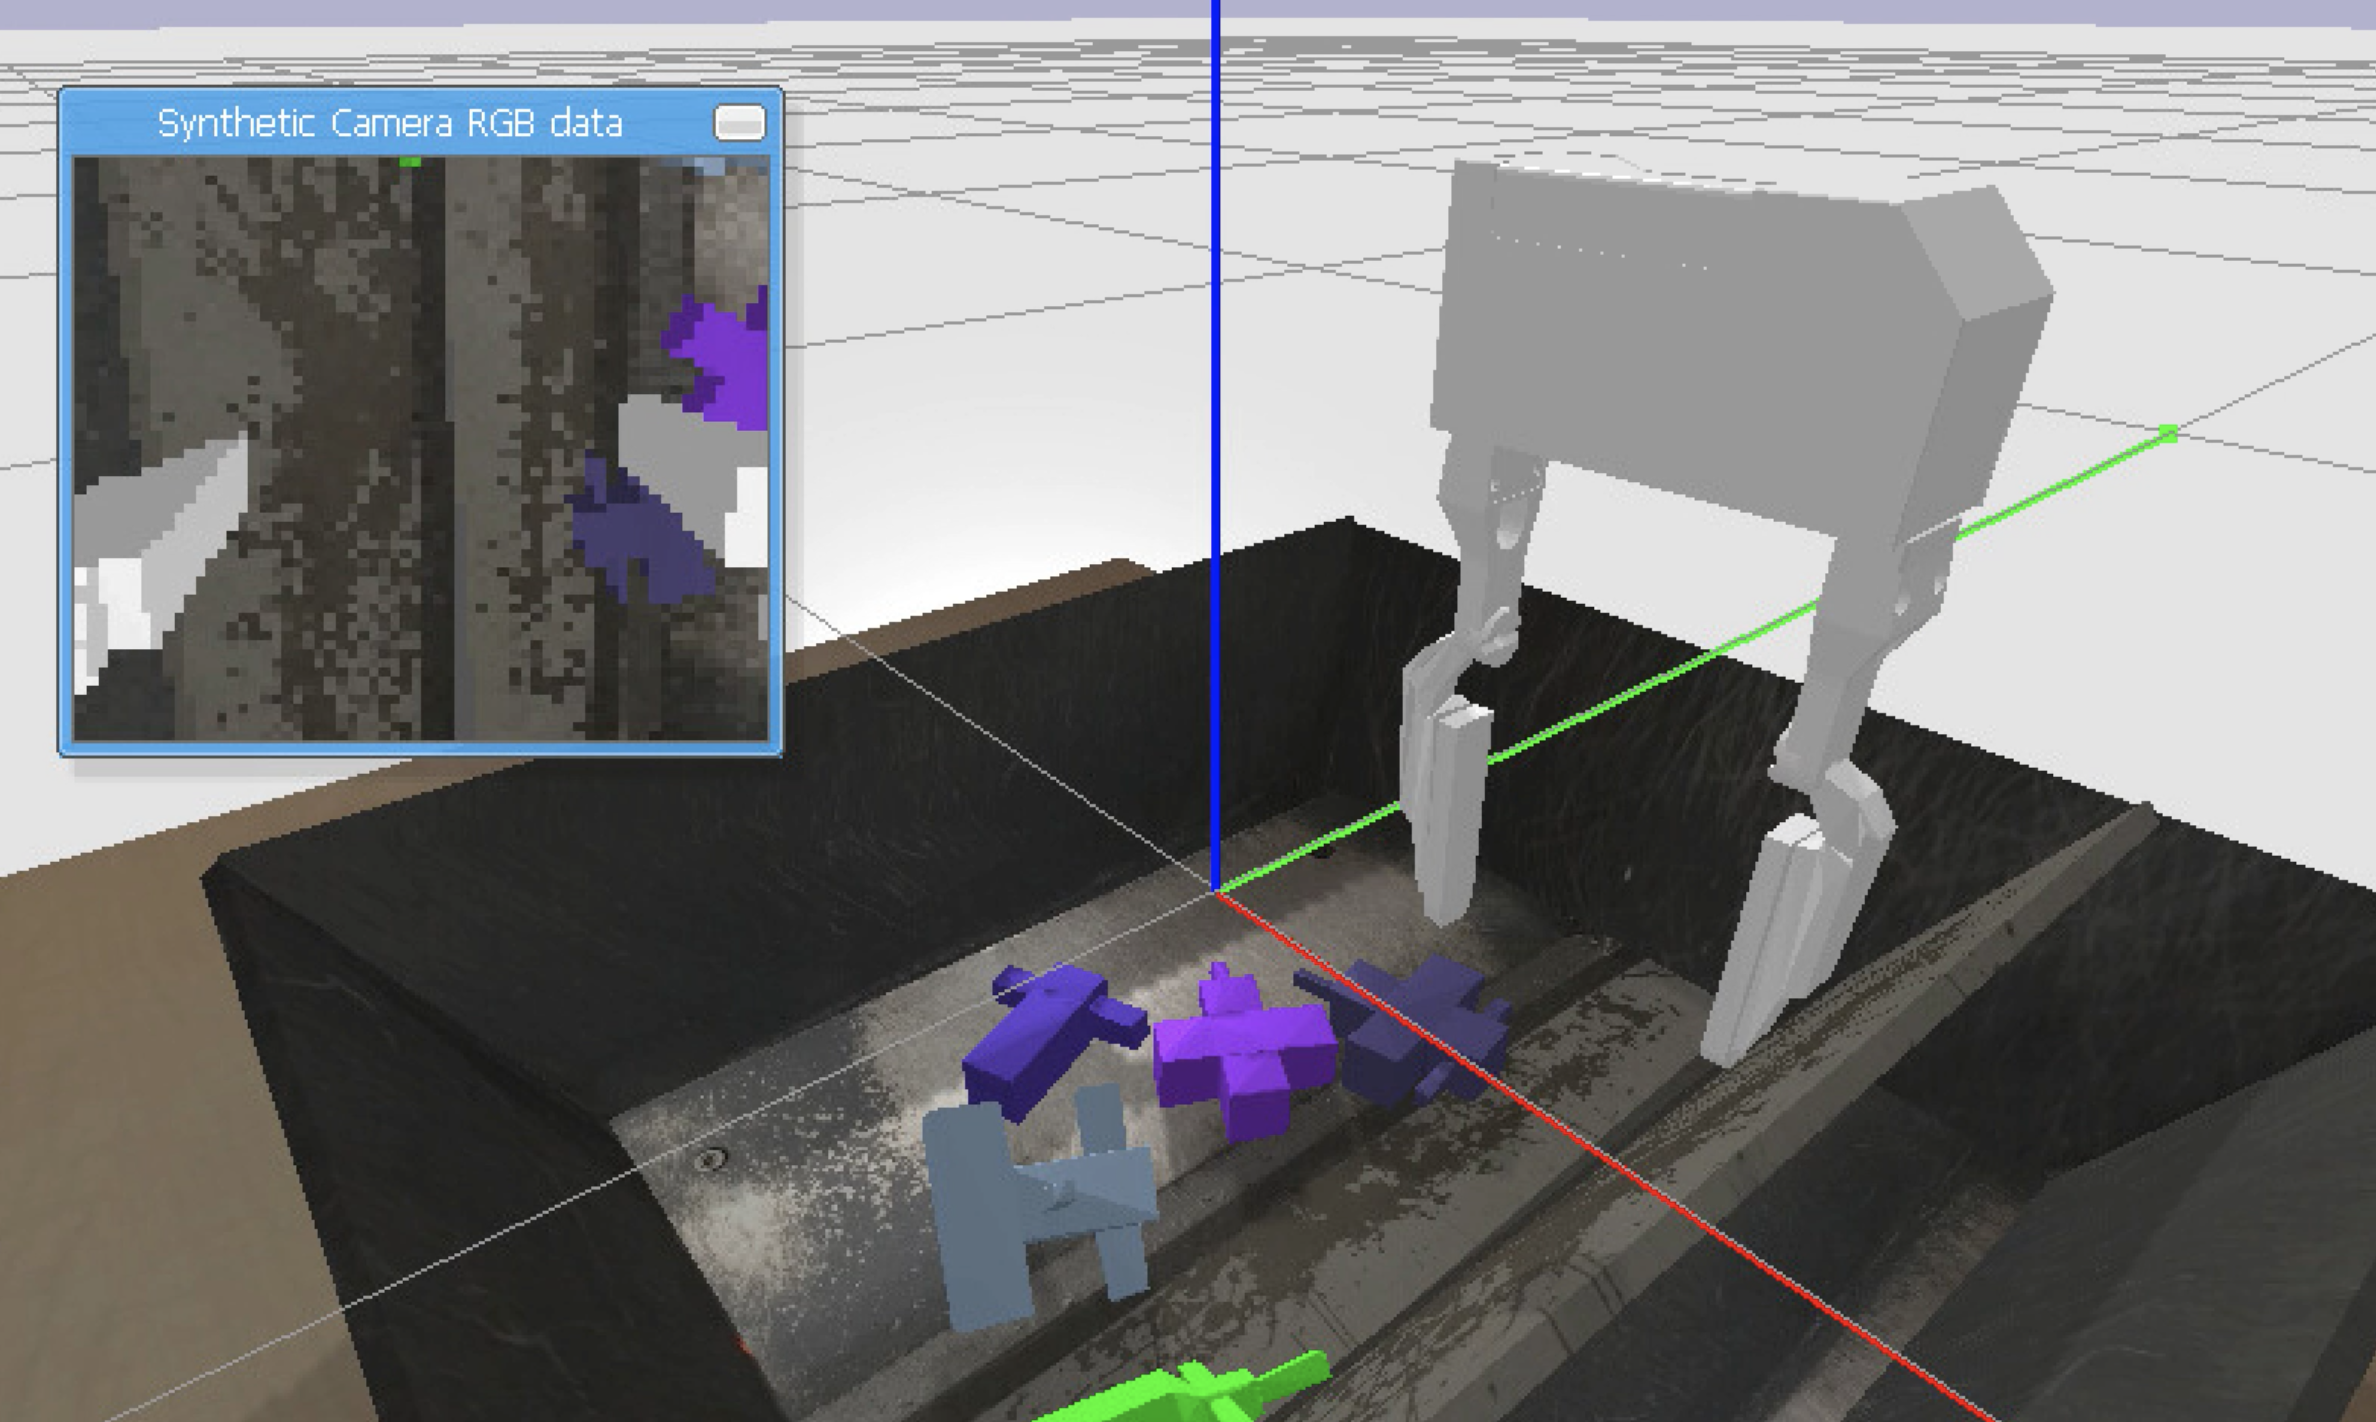
\includegraphics[width=\linewidth]{figures/failure/trayedge2}
            \caption{FGripper positions itself just above the tray's edge} \label{fig:floor}
        \end{subfigure}%
        \hspace*{\fill}   % maximize separation between the subfigures    
        \begin{subfigure}{0.33\textwidth}
            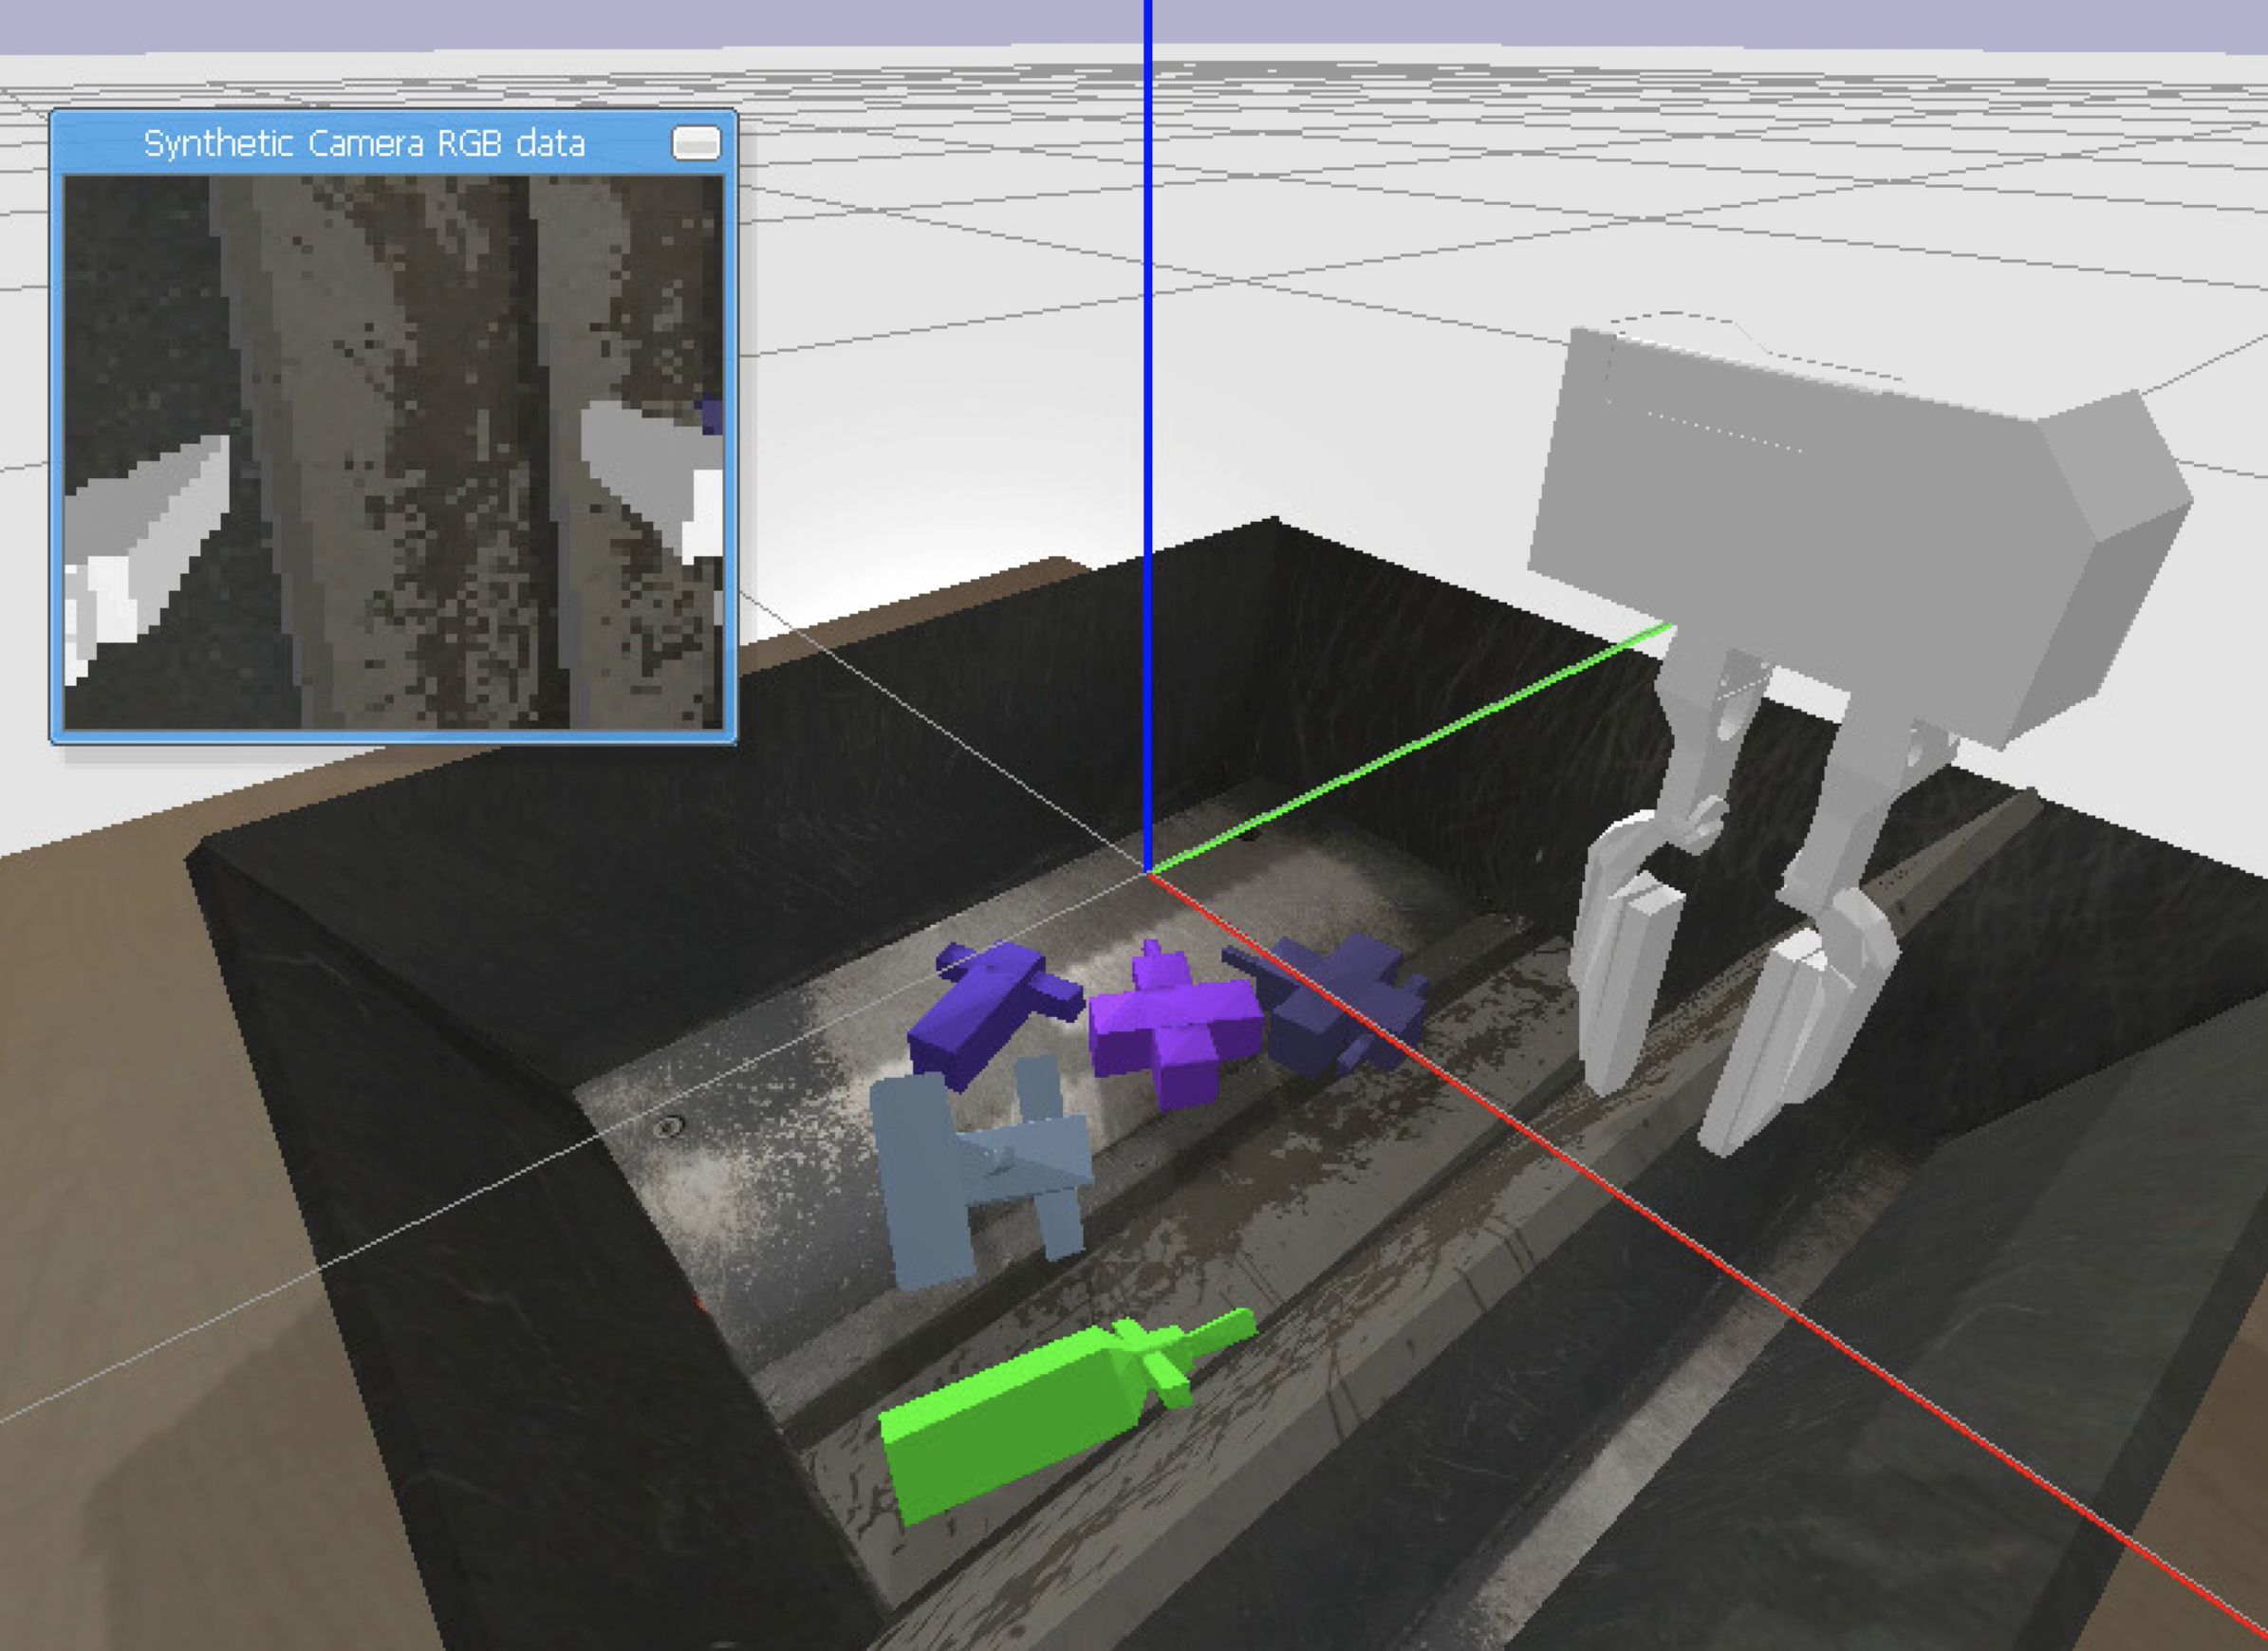
\includegraphics[width=\linewidth]{figures/failure/trayedge3}
            \caption{Gripper grasps the tray's edge} \label{fig:floor}
        \end{subfigure}%
        \hspace*{\fill}   % maximize separation between the subfigures    
        \caption{Sequence of movement to the tray's edge\label{fig:failTrayEdge}}
    \end{figure} 

\end{enumerate}

% \section{DQN vs. BDQ}

% \section{Encoder vs. Raw Sensor Input}

% \section{Ablation Studies}

% \subsection{Curriculum Strategy}

% \subsection{Normalization}

% \subsection{Shaped Reward}

% \subsection{Actuator Width}

% \section{Failure Modes}

